\documentclass[lang=cn,11pt,chinesefont=nofont]{elegantbook}

% 字体配置:
% macOS:   fontset=macnew  或 fontset=mac
% Windows: fontset=windowsnew 或 fontset=windows
% Linux:   fontset=ubuntu 或 fontset=fandol
% 如果注释掉 fontset,ctex 会尝试自动检测系统字体
%\usepackage[UTF8,scheme=plain,fontset=macnew]{ctex}
\usepackage[UTF8,scheme=plain]{ctex}
% 显式设置中文字体,确保 \textbf 对中文可见(Linux 友好)
\setCJKmainfont{FandolSong-Regular}[BoldFont=FandolSong-Bold,AutoFakeBold=2]
\setCJKsansfont{FandolHei-Regular}[AutoFakeBold=2]
\setCJKmonofont{FandolFang-Regular}[AutoFakeBold=2]






\title{Math 525}

\begin{document}
\frontmatter
\tableofcontents
\mainmatter

% 包含各个章节
% \input{chapters/01-basic-combinatorics}
% \chapter{Probability space intro}
\section{probability space}
我们这里跳过所有 measure theory 的内容, 见 notes on measure theory.\\
\begin{definition}{prob space, prob measure, sample space, event space}
    一个 probability space 就是一个 measure space \( (\Omega, \mathcal{F}, \mathbb{P}) \), 其中 $\mathbb{P}(\emptyset) =0, \mathbb{P}(\Omega) = 1$.\\
    对于这样的 measure $\mathbb{P}$, 我们称之为 \textbf{probability measure (概率测度, 即概率)}.\\
    而这里的 \(\Omega\) 我们称之为 \textbf{sample space (样本空间)}; 这里的 $\sigma$-algebra $\mathcal{F}$, 我们称之为 \textbf{event space (事件空间)}. \\
    任意的 $A \subset \Omega$ 都是一个 \textbf{event}, 但是概率论中只考虑 $A\in\mathcal{F}$, 即 measurable event. 为简化, event 这个单词就指 measurable event.
\end{definition}
\begin{remark}
    回顾一下 measure space 的定义:
    \begin{itemize}
        \item 一个 set $\Omega$ 的一个 $\sigma$-algebra 就是一个包含空集的子集簇, 其 \textbf{closed under countable unions and complements}. (如果只 closed under finite unions, 则只称为一个 algebra.)
        \item 一个 Borel algebra 是一个定义在 topological space 上的 $\sigma$-algebra, 由 all open sets 生成. (因而: closed under countable unions and complements.) $\mathbb{R}$ 的 Borel algebra 可以由 all open intervals 生成.
        \item 一个 measure on a measurable space $(\Omega, \mathcal{F})$ 就是一个从 $\mathcal{F} \to \mathbb{R}$ 的函数, 满足 \textbf{countable additivity}.
        \item measure 的性质: \textbf{(1)non-negativity, (2) monotonicity, (3) countable subadditivity, (4) inclusion-exclusion principle (上节已讲), (5) continuity from below and above.} 第 (5) 条具体即:
        For measurable sets $A_1 \subseteq A_2 \subseteq \cdots \subseteq A_n \subseteq \cdots$, then $\lim_{n \to \infty} \mathbb{P}(A_n) = \mathbb{P}(\bigcup_{n=1}^{\infty} A_n)$.\\
        For measurable sets $A_1 \supseteq A_2 \supseteq \cdots \supseteq A_n \supseteq \cdots$, then $\lim_{n \to \infty} \mathbb{P}(A_n) = \mathbb{P}(\bigcap_{n=1}^{\infty} A_n)$.
    \end{itemize}
\end{remark}
\begin{remark}
    对于 discrete 的 prob space 而言, 通常选取 $\mathcal{F} = 2^{\Omega}$, 即 $\Omega$ 的任意子集都是一个 event.
\end{remark}
\begin{remark}
    概率空间的现实意义是: 一次 experiment 的所有可能的结果的集合, 以及每个结果的概率.
    \begin{align*}
        \Omega &= \{\omega \mid \omega \text{ 是一次 experiment 的可能的结果}\}\\
        \mathbb{P}(\omega) &= \text{ 结果 $\omega$ 的可能性}
    \end{align*}
\end{remark}

\begin{example}
    (dice roll) 
    如果我们掷一个 6 面的骰子, 那么样本空间 $\Omega=\{1,2,3,4,5,6\}$. 一个可能的事件是 $A=\{1,2\}$. 如果假设骰子是公平的 (所有结果都是等可能的), 那么事件 $A$ 的概率是
    \[
    \mathbb{P}(A)=\frac{\text { Number of favorable outcomes }}{\text { Total number of outcomes }}=\frac{|A|}{|\Omega|}=\frac{2}{6} 
    \]
    % 如果我们定义一个随机变量 $X$ 表示掷骰子的结果, 那么 $X$ 的样本空间是 $\mathbb{R}$, 即 $X: \Omega \rightarrow \mathbb{R}$. 
    % 那么 $X$ 的分布函数是
    % \[
    % F_X(x) = \mathbb{P}(X \leq x) = \begin{cases}
    %     0, & x < 1 \\
    %     1/6, & 1 \leq x < 2 \\
    %     2/6, & 2 \leq x < 3 \\
    % \end{cases}
    % \]
    根据我们 measure-based 的定义, 这一结果自然 follows from countable additivity of $\mathbb{P}$.
\end{example}




\begin{example}
    三个人独立地掷一个 6 面的骰子, 求第三个人掷出的点数等于前两个人的点数之和的概率.
    \begin{solution}
        样本空间 $\Omega=\{1,2,3,4,5,6\}^3$.
        event: $E = \{ \omega \in \Omega \mid \omega_3 = \omega_1 + \omega_2 \}$.\\
        这个 event 有 15 个 elements: \[
        E = \{ (1,1,2), (1,2,3), (1,3,4), \cdots, (2,1,3), (2,2,4), \cdots, (3,1,4), \cdots, (4,1,5), \cdots, (5,1,6) \}
        \]
        因此, 概率是: \[
        \mathbb{P}(A)=\frac{|A|}{|\Omega|}=\frac{15}{216}=\frac{5}{72}
        \]
    \end{solution}
\end{example}


\begin{example}
    两个人计划在 12:00 到 1:00 之间碰面. 他们各自都会在期间的某个时间点到达. 求: 他们彼此不会等待对方超过 10 分钟的概率.\\
    \begin{solution}
        Sample space $$\Omega = \{(x,y): 0\leq x \leq 60, 0\leq y \leq 60\} = [0,60] \times [0,60]$$
        我们要求概率的事件 \[
        E = \{ (x,y)\in \Omega : |x-y| \leq 10 \} 
        \]
        容易画出图像:
        \begin{center}
        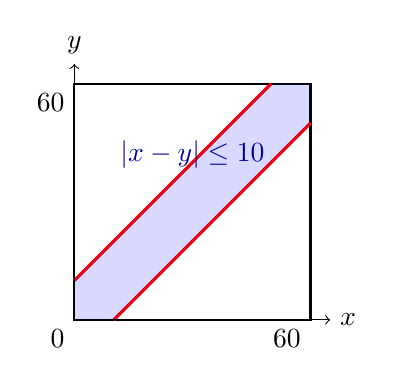
\begin{tikzpicture}[scale=0.05]
            % 绘制正方形区域
            \draw[thick] (0,0) rectangle (60,60);
            % 绘制两条界限直线: x-y=10  与 x-y=-10
            \draw[red,very thick] (10,0) -- (60,50);   % x - y = 10
            \draw[red,very thick] (0,10) -- (50,60);   % x - y = -10
            % 填充有效区域
            \fill[blue,opacity=0.15] 
                (0,10) -- (10,0) -- (60,50) -- (50,60) -- cycle;
            % 漏画了两个小的角
            \fill[blue,opacity=0.15]
                (0,0) -- (0,10) -- (10,0) -- cycle;
            \fill[blue,opacity=0.15]
                (60,60) -- (60,50) -- (50,60) -- cycle;
            % 坐标轴
            \draw[->] (0,0) -- (65,0) node[right] {$x$};
            \draw[->] (0,0) -- (0,65) node[above] {$y$};
            % 标注几个重要点
            \foreach \p/\lab in {(0,0)/0, (60,0)/60, (0,60)/60} {
                \draw \p node[below left]{\lab};
            }
            % 标签
            \node[blue!60!black] at (30,42) {$|x-y|\leq 10$};
        \end{tikzpicture}
        \end{center}
        因而概率是
        \[
        \mathbb{P}(E) = \frac{m(E)}{m(\Omega)} = \frac{3600-2500}{3600} = \frac{11}{36}
        \]
    \end{solution}
\end{example}



\section{conditional probability}
\begin{definition}{conditional probability}
    对于 probability space \((\Omega, \mathcal{F}, \mathbb{P})\), 给定一个 event $B \in \mathcal{F}$, 如果 \(\mathbb{P}(B) > 0\), 我们定义 conditional probability of an event $A \in \mathcal{F}$ given $B$ 为:
    \[
    \mathbb{P}(A \mid B) = \frac{\mathbb{P}(A \cap B)}{\mathbb{P}(B)}
    \]
\end{definition}
\begin{proposition}{decomposing probability of intersection of events}   
    令 $\left(A_i\right)_{i \in \mathbb{N}}$ 为一个 seq of events, 对于任意 $n \in \mathbb{N}$:
    \[
    \mathbb{P}\left(A_1 \cap A_2 \cap \ldots \cap A_n\right)=\mathbb{P}\left(A_1\right) \cdot \mathbb{P}\left(A_2 \mid A_1\right) \cdot \mathbb{P}\left(A_3 \mid A_1 \cap A_2\right) \ldots \cdot \mathbb{P}\left(A_n \mid A_1 \cap \ldots \cap A_{n-1}\right)
    \]
\end{proposition}
\begin{proof}
Naturally follows from the def. 
\end{proof}


\subsection{Law of total probability and Bayes' Theorem}
\begin{theorem}{law of total probability}
    令 $\left(A_i\right)_{i \in \mathbb{N}}$ 为一个 seq of \textbf{pairwise disjoint} events, 如果 $\sqcup_{i=1}^{\infty} A_i=\Omega$, 那么对于任意 event $E \subseteq \Omega$:
    \[
    \mathbb{P}(E)=\sum_{i=1}^{\infty} \mathbb{P}\left(A_i\right) \mathbb{P}\left(E \mid A_i\right)
    \]
\end{theorem}
\begin{proof}
    \[
    \mathbb{P}(E)=\mathbb{P}\left(E \cap \cup_{i=1}^{\infty} A_i\right)=\mathbb{P}\left(\cup_{i=1}^{\infty} E \cap A_i\right)=\sum_{i=1}^{\infty} \mathbb{P}\left(E \cap A_i\right)=\sum_{i=1}^{\infty} \mathbb{P}\left(A_i\right) \mathbb{P}\left(E \mid A_i\right)
    \]
\end{proof}
\begin{remark}
    \(P(A_i)P(E\mid A_i)\) 就等于 \(P(E \cap A_i)\), 也就是在 \(A_i\) 这个区域上, \(E\) 的 measure. 因而 disjoint union 之下就是 \(E\) 的完整 measure.
\end{remark}

\begin{theorem}{Bayes theorem}
    If $A, B \subseteq \Omega$ such that $\mathbb{P}(B) \neq 0$, then
    \[
    \mathbb{P}(A \mid B)=\frac{\mathbb{P}(A) \cdot \mathbb{P}(B \mid A)}{\mathbb{P}(B)}
    \]
\end{theorem}
\begin{remark}
    这其实是一个非常直接的结果, 因为 \(P(A) \dot P(B \mid A) = P(A \cap B)\). \\
    但是它的意义在于, 如果我们知道两个事件的概率和其中一个对另一个的条件概率, 我们就也得到了反过来的条件概率.
\end{remark}



\begin{example}{(Medical testing)}

在一个群体中, 随机选取一个人患有某种罕见疾病的概率是 0.001. 该疾病有一个诊断测试, 其性质如下: 给定个体患病, 测试呈阳性的概率 (真正阳性率) 是 0.99. 给定个体健康, 测试呈阳性的概率 (假阳性率) 是 0.02. 从群体中随机选取的一个人测试呈阳性. 该个体实际上患有该疾病的概率是多少?
于是
\begin{solution}
由 law of total probability, 我们有
\[
 \mathbb{P}(\text {positive})= \mathbb{P}(\text{positive} \mid \text{sick}) \mathbb{P}(\text{sick}) + \mathbb{P}(\text{positive} \mid \text{healthy}) \mathbb{P}(\text{healthy}) = 0.99 \cdot 0.001 + 0.02 \cdot 0.999 = 0.02097
\]
于是
\[
\mathbb{P}(\text {sick} \mid \text {positive})=\frac{0.99 \cdot 0.001}{0.02097} \approx 0.047
\]
\end{solution}
\end{example}

\begin{example}{(Monty Hall problem)}

假设你参加一个游戏节目, 面前有三扇门: 一扇门后面有一辆车; 其他两扇门后面是山羊. 你选择了一扇门, 比如说是 1 号门, 然后主持人打开了另一扇门, 比如说是 3 号门, 里面有一只山羊. 然后他说 "你想换成 2 号门吗?". 换门对你有利吗?
\begin{solution}
令 \(A_i\) 表示: car 在 \(i\) 号门后面; \(B\) 事件表示: 主持人打开 3 号门. 我们要求的概率是在事件 \(B\) 发生的情况下, \(A_2\) 的个概率, 即 \(\mathbb{P}(A_2 \mid B)\). 它的大小是:
\begin{align*}
\mathbb{P}(A_2 \mid B) &= \frac{\mathbb{P}(A_2) \cdot \mathbb{P}(B \mid A_2)}{\mathbb{P}(B)} \\
&= \frac{\mathbb{P}(B \mid A_2)\mathbb{P}(A_2)}{\mathbb{P}(B\mid A_1)\mathbb{P}(A_1) + \mathbb{P}(B\mid A_2)\mathbb{P}(A_2) + \mathbb{P}(B\mid A_3)\mathbb{P}(A_3)}    \\
&= \frac{1 \cdot \frac{1}{3}}{\frac{1}{2} \cdot \frac{1}{3} + 1 \cdot \frac{1}{3} + 0 \cdot \frac{1}{3}} = \frac{2}{3} > \frac{1}{3}
\end{align*}
因而, 换门是有利的.
\end{solution}
\begin{remark}
这是一个非常反直觉的例子. 我们直觉肯定会觉得: 一共 1 辆车和 2 个山羊, 主持人帮忙排除掉了一个山羊, 
那么剩下来的两个里面我们二选一, 肯定是 $1/2$ 概率, 而这个 "更换与否" 就是二选一的抉择. 但其实不是这样的. \\
在第一次选择和第二次选择之间, 主持人带来了额外的信息. 
\begin{itemize}
    \item 不换门: win iff 在一开始就选择对了车, 这个概率是 $1/3$.
    \item 换门: win iff 在一开始选择的是山羊, 这个概率是 $2/3$.
\end{itemize}
从条件概率的视角来看: 
\begin{itemize}
    \item 如果车在 2 号门: 主持人在这个环节里只能选择 3 号门.
    \item 如果车在 1 号门: 主持人在这个环节里可以随机在 2 号和 3 号门里面选择一扇门.
\end{itemize}
也就是说, 主持人打开 3 号门的这个动作, 把 3 号门原本含有的 "中奖潜力" 全部转移给了 2 号门.
这很反直觉. 但是可以用一段 python 程序验证:

\begin{python}[caption={Monty Hall problem simulation}, label=code:montyhall-sim]
import random

def monty_hall_sim(trials=10000):
    stay_wins = 0
    switch_wins = 0

    for _ in range(trials):
        # 1. 初始化门: 0代表羊, 1代表车
        doors = [0, 0, 0]
        car_position = random.randint(0, 2)
        doors[car_position] = 1
        
        # 2. 玩家最初的选择
        player_choice = random.randint(0, 2)
        
        # 3. 主持人打开一扇有山羊的门
        # 主持人不能开玩家选的门,也不能开有车的门
        possible_host_doors = [
            i for i in range(3) 
            if i != player_choice and doors[i] == 0
        ]
        host_opens = random.choice(possible_host_doors)
        
        # 4. 如果"坚持不换"赢了
        if doors[player_choice] == 1:
            stay_wins += 1
            
        # 5. 如果"换门"赢了
        # 换门后的选择是:既不是原选,也不是主持人开的那扇
        remaining_door = [
            i for i in range(3) 
            if i != player_choice and i != host_opens
        ][0]
        
        if doors[remaining_door] == 1:
            switch_wins += 1

    print(f"总实验次数: {trials}")
    print(f"坚持不换中奖次数: {stay_wins} (概率: {stay_wins/trials:.2%})")
    print(f"换门后中奖次数: {switch_wins} (概率: {switch_wins/trials:.2%})")

if __name__ == "__main__":
    monty_hall_sim()
\end{python}
运行结果:

\begin{terminal}[caption={Monty Hall problem simulation result}]
总实验次数: 10000  
坚持不换中奖次数: 3312 (概率: 33.12%)
换门后中奖次数: 6688 (概率: 66.88%) 
\end{terminal}
\end{remark}
\end{example}



\begin{example}{(Wizards)}

两个巫师 \(A\) 和 \(B\) 进行决斗, 他们轮流射击对方. 巫师 \(A\) 每次射击命中 \(B\) 的概率是 \(\mathbb{P}(A)=\frac{1}{2}\), 而巫师 \(B\) 每次射击命中 \(A\) 的概率是 \(\mathbb{P}(B)=\frac{2}{3}\). 巫师 \(A\) 先开枪. 求: 巫师 \(A\) 获胜的概率是多少? \\
\begin{solution}
任意一轮射击 (假设前一轮没有结束, 于是游戏回到初始状态. 因而任意一轮都是独立的) 中,
令 \(W_A\) 为事件: \(A\) 获胜; \(W_B\) 为事件: \(B\) 获胜, 假设他们从各自开始射击. 根据全概率公式, 我们有
$$
\begin{aligned}
& \mathbb{P}\left(W_A\right)=\mathbb{P}(\mathrm{hit}) \mathbb{P}\left(W_A \mid \mathrm{hit}\right)+\mathbb{P}(\mathrm{miss}) \mathbb{P}\left(W_A \mid \mathrm{miss}\right)=\frac{1}{2}+\frac{1}{2} \mathbb{P}\left(W_B^c\right) \\
& \mathbb{P}\left(W_B\right)=\mathbb{P}(\mathrm{hit}) \mathbb{P}\left(W_B \mid \mathrm{hit}\right)+\mathbb{P}(\mathrm{miss}) \mathbb{P}\left(W_B \mid \mathrm{miss}\right)=\frac{2}{3}+\frac{1}{3} \mathbb{P}\left(W_A^c\right)
\end{aligned}
$$
Solving the system, we find $\mathbb{P}\left(W_A\right)=0.6$.
\end{solution}
\begin{remark}
这个例子表明了先手优势有多大. 相比上一个例子, 这是很直观的.\\
另外, 这个例子有趣的是, 我们把无限的回合转化为了一个循环结构, 利用游戏状态的自相似, 只需要考虑任意一轮即可.
\end{remark}    
\end{example}

\subsection{Kolmogorov definition of conditional probability}
我们通过 \(\mathbb{P}(A \mid B) = \frac{\mathbb{P}(A \cap B)}{\mathbb{P}(B)}\) 定义出来的 conditional probability 有一个限制, 就是 enforce \(\mathbb{P}(B) > 0\). \\
但是, 难道 \(\mathbb{P}(B) = 0\) 就不能定义条件概率了吗? 我们考虑一个连续情况: 在 \(\mathbb{R}^3\) 中任意选择一个点, 求: 该点位于单位球面上的概率. 显然, 这个概率是 0. 但是, 如果我们知道该点位于单位球内, 那么该点距离原点的距离为 \(1\) 的概率应当为 \(1\). 也就是说,  即使在 \(\mathbb{P}(B) = 0\) 的情况下, 我们也希望定义 \(\mathbb{P}(A \mid B)\).\\
在考虑这个定义之前, 首先我们发现: 基于我们先前定义的 conditional probability, 我们可以获得一个新的 probability space:
\begin{definition}{conditional probability space and trace $\sigma$-algebra}
    对于给定的 prob space \((\Omega, \mathcal{F}, \mathbb{P})\), 给定一个 event \(B \in \mathcal{F}\) 且 \(\mathbb{P}(B) > 0\), 我们定义 conditional probability space as the triplet \((B, \mathcal{F}_B, \mathbb{P}(\cdot \mid B))\), 其中:
    \[
    F_B := \{A\cap B \mid  A \in \mathcal{F} \}
    \]
    被称为 \textbf{trace \(\sigma\)-algebra on \(B\)}.\\
    容易验证, 这个 triplet 是一个 prob space.
\end{definition}
\begin{remark}
    当我们把整个 prob space 限制在 event \(B\) 上时, 本质上是在做一个 Radon-Nikodym derivative 的操作.\\
    定义 \(f:= \frac{\mathbb{I}_B}{\mathbb{P}(B)}\), 那么对于任意 event \(A \in \mathcal{F_B}\), 有:
    \[
    \mathbb{P}(A \mid B) = \int_{A} f \, d\mathbb{P}
    \] 
    因而和我们的直觉一样, 条件概率是通过一个 density function 来重新加权原本的概率测度. 
\end{remark}
既然这样, 我们能否直接从一个新的 prob space \((B, \mathcal{F}_B, \mathbb{P}(\cdot \mid B))\) 出发, 来定义条件概率呢? 这就是 Kolmogorov 的定义:
\begin{definition}{Kolmogorov definition of conditional probability}
    对于给定的 prob space \((\Omega, \mathcal{F}, \mathbb{P})\), 
    设 \(\mathcal{G} \subseteq \mathcal{F}\) 是一个 sub-\(\sigma\)-algebra. 对于 event \(A \in \mathcal{F}\), 条件概率 \(\mathbb{P}(A \mid \mathcal{G})\) 是一个 \(\mathcal{G}\)-measurable 的随机变量, 其满足对于任意 \(G \in \mathcal{G}\), 有:
    \[
    \int_G \mathbb{P} (A \mid \mathcal{G}) \, d\mathbb{P} = \mathbb{P}(A \cap G)
    \]
    显然, 当 \(\mathbb{P}(B) > 0\) 时, 这个定义和我们之前的定义是等价的.\\
    这个 random variable \(\mathbb{P}(A \mid \mathcal{G})\) 在 \(\mathbb{P}\)-a.s. 意义下是唯一的.
\end{definition}
\begin{remark}
    条件概率 \(\mathbb{P}(A \mid \mathcal{G})\) 这个测度是 \(\mathbb{P}(A \cap \cdot)\) 这个测度相对于背景测度 \(\mathbb{P}\) 在子信息流 \(\mathcal{G}\) 下的 Radon-Nikodym derivative, 也就是一个密度函数. \\
    这个定义里没有指明, 给定一个 event \(B \in \mathcal{F}\), 如何去确定 \(\mathcal{G}\) 以及 \(\mathbb{P}(A \mid \mathcal{G})\). 虽然这是一个抽象的存在性 \(\&\) 唯一性定义, 但是标准的做法是:
    \begin{itemize}
        \item  看向产生 \(B\) 的 random variable \(X\), 即 \(B = \{X = x\}\), 令 \(\mathcal{G} = \sigma(X)\), 即由 random variable \(X\) 生成的 \(\sigma\)-algebra. 这个 \(\sigma\)-algebra 包含了所有关于 \(X\) 可能取值的信息.
        \item 既然 $\mathbb{P}(A \mid \sigma(X))$ 是关于 $\sigma(X)$ 可测的, 那么它一定可以写成 $h(X)$ 的形式. 通过对 $X$ 的所有可能取值进行积分, 我们确定了函数 $h(\cdot)$ 的整体形态, 这时我们定义 $P(A \mid X=x)$ 为函数 $h$ 在点 $x$ 处的值.
        \item \(\mathbb{P}(A \mid \mathcal{G})\) 实际就是条件期望 \(\mathbb{E}[\mathbb{I}_A \mid \mathcal{G}]\). 当 \(\mathbb{P}(B) > 0\) 时, 它就退化回经典定义 \( \frac{\mathbb{P}(A \cap B)}{\mathbb{P}(B)}\).
    \end{itemize}
\end{remark}
\begin{remark}
    Further issue: \textbf{Borel-Kolmogorov paradox}.\\
    即便是这个定义, 也会出现问题. \\
    给定一个事件 $B$, 如果 $\mathbb{P}(B)=0$, 则 $\mathbb{P}(A \mid B)$ 的取值取决于我们将 $B$ 嵌入到哪一个随机变量 $X$ 中.
不同的随机变量 $X, Y$ 即使都能产生相同的事件 $\{X=x\} = \{Y=y\} = B$, 它们生成的子 $\sigma$-代数 $\sigma(X)$ 和 $\sigma(Y)$ 却不同, 导致最终确定的条件概率 $h_X(x) \neq h_Y(y)$. \\
为了解决这个问题, 可以引入更精细的结构, 比如说 regular conditional probability, 以及 disintegration theorem. 不过此处不展开了.
\end{remark}

\section{independence}
\begin{definition}{independence of events}
    对于 prob space \((\Omega, \mathcal{F}, \mathbb{P})\), 两个 events \(A, B \in \mathcal{F}\) 如果有
    \[
    \mathbb{P}(A \cap B) = \mathbb{P}(A) \cdot \mathbb{P}(B)
    \]
    则称 \(A\) 和 \(B\) 是 independent 的.\\
    更加 generally, 对于任意 collection of events \(\{A_i\}_{i \in I}\), 如果对于任意有限子集 \(J \subseteq I\), 有 
    \[
    \mathbb{P}\left(\bigcap_{j \in J} A_j\right) = \prod_{j \in J} \mathbb{P}(A_j)
    \]
    则称 \(\{A_i\}_{i \in I}\) 是 mutually independent 的.
\end{definition}
\begin{remark}
    根据条件概率的定义, 容易得出: 两个 events \(A, B\) independent 的定义\textbf{等价于 \(\mathbb{P}(A \mid B) = \mathbb{P}(A)\)}, 即事件 \(B\) 的发生与否不影响事件 \(A\) 发生的概率.\\
    将它推广到多个事件: 即\textbf{任意一个事件的发生与否都不影响其他事件发生的概率}.
\end{remark}

\begin{proposition}
    如果 events \(A\) 和 \(B\) independent, 则 \(A\) 和 \(B^c\) 也是 independent 的.
\end{proposition}
\begin{proof}
\[
\begin{aligned}
\mathbb{P}\left(A^c \cap B^c\right) & =\mathbb{P}\left((A \cup B)^c\right)=1-\mathbb{P}(A \cup B)=1-\mathbb{P}(A)-\mathbb{P}(B)+\mathbb{P}(A \cap B) \\
& =1-\mathbb{P}(A)-\mathbb{P}(B)+\mathbb{P}(A) \cdot \mathbb{P}(B) = (1-\mathbb{P}(A))(1-\mathbb{P}(B)) \\
& =\mathbb{P}\left(A^c\right) \cdot \mathbb{P}\left(B^c\right)
\end{aligned}
\]
\end{proof}


\begin{example}{(Pairwise Independence vs. Mutual Independence)}

一组事件 $A_1, A_2, \ldots \in \mathcal{F}$ 如果是 mutually independent 的, 则它们两两 independent. \textbf{但是反过来不成立}.\\
即: \textbf{即便对于任意 $i \neq j$, 有 $\mathbb{P}(A_i \cap A_j) = \mathbb{P}(A_i) \mathbb{P}(A_j)$, 也并不意味着这些事件是 mutually independent 的}.\\
下面为一个 counterexample: 考虑掷两个骰子. 令事件
$$
A:=\{\text{first roll is } 4\}, \quad B:=\{\text{second roll is } 3\},\quad C:=\{\text{the sum of the two outcomes is } 7\}
$$
我们发现: $\mathbb{P}(A \cap B \cap C)=\frac{1}{36} \neq \mathbb{P}(A) \mathbb{P}(B) \mathbb{P}(C)=\frac{1}{6^3}$, 因而 $A, B, C$ 并不 mutually independent. 然而, However, $\mathbb{P}(A \cap B)=\frac{1}{36}=\mathbb{P}(A) \mathbb{P}(B), \mathbb{P}(A \cap C)=\frac{1}{36}=\mathbb{P}(A) \mathbb{P}(C)$ and $\mathbb{P}(B \cap C)=\frac{1}{36}=\mathbb{P}(B) \mathbb{P}(C)$, 
因而它们两两 pairwise independent.
\end{example}
\begin{remark}
这个反例能够成功的理由是: 事件 $C$ (总和) 和 事件 $A$ (第一个骰子) 以及事件 $B$ (第二个骰子) 分别都是独立的, 因为知道了其中一个并不会影响另一个的概率. 但是, 一旦我们知道了 $A$ 和 $B$ 的值, 那么 $C$ 的值就被完全确定了 (因为总和就是两个骰子的和). 因而, 三个事件并不 mutually independent. \\
(注意: 如果 \(C\) 事件不是和为 7 而是一个小于 7 的数, 那就不是了, 因为如果我们知道第一次是 6, 那么和就不可能是 6, 那么就也失去了 pairwise independence).\\
这个例子说明了, mutual independence 是一个比较强的条件.
我们可以把这三个事件看作是对结果空间的约束:
\begin{itemize}
    \item 两个骰子的结果空间有 36 个点.
    \item $A$ 是一条线 (6个点), $B$ 是另一条线 (6个点), $C$ 是一条对角线 (6个点)。
    \item 两两独立: 意味着任意两条线相交的点数, 恰好符合概率乘积.
    \item 相互独立: 要求这三条线交于一点的概率也符合乘积. 
\end{itemize}
这个例子提醒我们: 独立性不是一种可以由低维向高维简单“归纳”的性质. 一个系统可以局部解耦(两两独立, 但在全局尺度上却存在强耦合. 总之 mutual independence 是一个很强的条件.
\end{remark}



\begin{example}{(coin tossing)}

假设我们有一枚不均匀的硬币, 掷出正面的概率是 $p \in[0,1]$, 反面的概率是 $1-p$. 我们不断地掷这枚硬币, 直到第一次掷出正面为止, 并记录所需的掷币次数. 求: 掷币次数为奇数的概率是多少?
\begin{solution}
对于任意 $i \in \mathbb{N}$, 考虑事件 $A_i=\{$ 掷币次数为 $i\}$.
$$
\mathbb{P}\left(\cup_{n=1}^{\infty} A_{2 n-1}\right)=\sum_{n=1}^{\infty} \mathbb{P}\left(A_{2 n-1}\right)=\sum_{n=1}^{\infty}(1-p)^{2 n-2} p=p \sum_{n=1}^{\infty}\left((1-p)^2\right)^{n-1}=p \cdot \frac{1}{1-(1-p)^2}=\frac{1}{2-p}
$$
\end{solution}
\begin{remark}
这个问题还可以通过 law of total probability 来解决.\\
令 $E=$ 掷币次数为奇数. 那么
$$
\begin{aligned}
\mathbb{P}(E) & =\mathbb{P}(\text{head}) \cdot \mathbb{P}(E \mid \text{head})+\mathbb{P}(\text{tail}) \cdot \mathbb{P}(E \mid \text{tail}) \\
& =p \cdot 1+(1-p) \cdot(1-\mathbb{P}(E))
\end{aligned}
$$
Solve 这个 equation 得到同样结果.
\end{remark}    
\end{example}
% \chapter*{Homework 1}



\section*{Problem 1}
Let $n \in \mathbb{N}$.
\begin{itemize}
    \item[(a)] Show that $2^n=\sum_{k=0}^n\binom{n}{k}$. Given that a set of $n$ elements has $2^n$ subsets, what is the combinatorial interpretation of this equality?
    \item[(b)] Show that $$\sum_{k \text { odd }, 0 \leq k \leq n}\binom{n}{k}=\sum_{k \text { even }, 0 \leq k \leq n}\binom{n}{k} $$
    \item[(c)] Show that $$\binom{2 n}{n}=\sum_{k=0}^n\binom{n}{k}^2 $$
\end{itemize}
Hint: You may use $\binom{n}{k}^2=\binom{n}{k}\binom{n}{n-k}$.
\begin{proof}
    \begin{itemize}
        \item[(a)] 
By the binomial theorem, we have:
\[
(1+1)^n = \sum_{k=0}^n \binom{n}{k} 1^k 1^{n-k} = \sum_{k=0}^n \binom{n}{k}
\]
The combinatorial interpretation of this equality is that:
Let $S_k$ be the collection of all subsets that have size $k$.
For collection $S_k$, its size is $\binom{n}{k}$ since it represents choosing $k$ elements from $n$ elements without regard to order.\\
Therefore the total number of subsets of $S$ is:
\[
| \mathcal{P}(S) |=\sum_{k=0}^n |S_k|  =\sum_{k=0}^n \binom{n}{k} =2^n
\]        
        \item[(b)] 
Using the binomial theorem, we have:
\[
0 = (1-1)^n = \sum_{k=0}^n \binom{n}{k} (-1)^k 1^{n-k} = \sum_{k=0}^n \binom{n}{k} (-1)^k
\]
Thus:
\begin{align}
    &\quad\quad\quad\quad \sum_{k=0}^n \binom{n}{k} (-1)^k = 0 \nonumber \\
    &\implies \sum_{0\leq k \leq n,\, k \text{ odd} } \binom{n}{k} (-1)
    + \sum_{0\leq k \leq n,\, k \text{ even} } \binom{n}{k} (1) = 0 \nonumber \\
    &\implies \sum_{0\leq k \leq n,\, k \text{ odd} } \binom{n}{k}
    = \sum_{0\leq k \leq n,\, k \text{ even} } \binom{n}{k}
\end{align}
        \item[(c)] 
We prove by combinatorial argument.\\
Let $S$ be a setwith $2n$ distinct elements. The number of ways to choose a subset $P$ containing $n$ elements is $\binom{2n}{n}$.\\
In another way: 
We can first arbitrarily divide the $2n$ distinct elements into two groups: group $A$ and group $B$, each containing $n$ elements:
\[
S = A \sqcup B
\]
And fix the two groups. \\
For any subset $P$ of the $2n$ elements with size $n$, some of them are from group $A$, and the rest of them are from group $B$. \\
Let $k$ be the number of elements of $P$ that are chosen from $A$, then the number of elements chosen from $B$ must be $n-k$.\\
Note the number of ways to choose $k$ elements from $A$ is $\binom{n}{k}$, and the number of ways to choose $n-k$ elements from $B$ is $\binom{n}{n-k}$. \\
Therefore, the total number of ways to get $P$ from $S=A \sqcup B$ with $k$ elements from $A$ is $\binom{n}{k}\binom{n}{n-k} = \binom{n}{k}^2$.\\
Thus, summing over all possible values of $k=0,1,\dots,n$, the number of ways to choose $n$ elements from $S$ i.e. the number of ways to get $P$ from $S$, is $$\sum_{k=0}^n \binom{n}{k}^2$$
Thus, we obtain $$\binom{2n}{n}=\sum_{k=0}^n \binom{n}{k}^2$$ as desired.
    \end{itemize}
\end{proof}


\section*{Problem 2}
We roll a fair die three times and record the outcomes $a, b, c \in\{1,2,3,4,5,6\}$. What is the probability that the equation $a x^2+b x+c=0$ does not have solutions in the real numbers?
\begin{solution}
    The equation $a x^2+b x+c=0$ does not have solutions in the real numbers iff the the discriminant is negative, i.e. $\Delta=b^2-4 a c<0$.\\
    Total possible equations is $6^3 = 216$. For each $b$, the total possible $(a,c)$ pairs are $36$. We can calculate the number of $(a,c)$ pairs that satisfy the condition case by case.
\begin{itemize}
\item For $b=1$: $4ac > 1$ holds for all $(a,c)$.
\item For $b=2$: $4ac > 4 \implies ac > 1$, which excludes only $(1,1)$.
\item For $b=3$: $4ac > 9 \implies ac \ge 3$ since they are integers, so excluding $(1,1),(1,2),(2,1)$ ($3$ cases).
\item For $b=4$: $4ac > 16 \implies ac \ge 5$, excluding: $(1,3),(1,4),(2,2),(3,1),(4,1)$ besides the previous case, thus $8$ cases excluded.
\item For $b=5$: $4ac > 25 \implies ac \ge 7$, excluding: $(1,5),(1,6),(2,3),(3,2),(5,1),(6,1)$ besides the previous case, thus $14$ cases excluded.
\item For $b=6$: $4ac > 36 \implies ac \ge 10$, excluding: $(2,4),(3,3),(4,2)$ besides the previous case, thus $17$ cases excluded.
\end{itemize}
Thus, the total number of triples for which the discriminant is not negative (exlcuded) is
\[
1+ 3 + 8 + 14 + 17 = 43
\]
Therefore, the desired probability is
\[
1-\mathbb{P}(\text{the equation has solutions in the real numbers}) = 1-\frac{43}{216} = \frac{173}{216}
\]
\end{solution}


\section*{Problem 3}
An ant starts at the origin $(0,0)$ on the integer lattice.
At each step it moves either one unit to the right or one unit upward, each with probability $\frac{1}{2}$. 
The ant continues moving until it reaches the point $(205,200)$.\\
What is the probability that the ant visits the point $(105,100)$ at some time during its journey?\\
Hint: Start by counting the number of paths from $(0,0)$ to $(205,200)$.
\begin{solution}
Any path from $(0,0)$ to $(205,200)$ must consist of $205$ steps to the right and $200$ steps upward, for a total of $405$ steps. 
So a path is uniquely determined by the choice of 205 steps to the right (which is equivalent to the choice of 200 steps upward).\\
Thus total number of paths from $(0,0)$ to $(205,200)$ is
\[
N = \binom{405}{205}
\]

A path passes through the point $(105,100)$ if and only if it first goes from $(0,0)$ to $(105,100)$ and then from $(105,100)$ to $(205,200)$.\\
Thus the number of such paths is the product of the number of paths from $(0,0)$ to $(105,100)$ and the number of paths from $(105,100)$ to $(205,200)$, by the fundamental counting principle.
For the same reason as deciding the number of total paths from $(0,0)$ to $(205,200)$, the number of paths from $(0,0)$ to $(105,100)$ is
\[
N_1 = \binom{205}{105}
\]
And similarly, the number of paths from $(105,100)$ to $(205,200)$ is
\[
N_2 = \binom{200}{100}
\]
Note that from a point to another point, all such paths are equally likely to be chosen. Therefore, the desired probability is
\[
\mathbb{P}(\text{path passes through $(105,100)$}) = \frac{\binom{205}{105}\binom{200}{100}}{\binom{405}{205}}
\]
\end{solution}

\section*{Problem 4}
From a lottery containing $n$ tickets numbered $1,2, \ldots, n$, a ticket is drawn, its number is recorded, and then it is returned to the lottery. This process is repeated $k \geq 3$ times. Find the probabilities of the following events:
\begin{itemize}
    \item[(a)] Ticket 1 is selected at least once.
    \item[(b)] Tickets 1, 2, and 3 are each selected at least once.
\end{itemize}
\begin{solution}
\begin{itemize}
    \item[(a)] 
 Let $E$ be the event that ticket $1$ is selected at least once.
 \begin{align*}
    \mathbb{P}(E) &= 1 - \mathbb{P}(\text{ticket $1$ is never selected in $k$ draws}) \\
    &= 1 - \left(\frac{n-1}{n}\right)^k \tag*{\text{(by independence of each draw)}}
 \end{align*}
    \item[(b)] 
Let $F$ be the event that tickets $1,2,3$ are each selected at least once. \\
For $i=1,2,3$, let
\[
A_i:=\{\text{ticket } i \text{ is never selected in the } k \text{ draws}\}
\]
Thus 
\[
P(F) = 1 - P(A_1 \cup A_2 \cup A_3)
\]
By the principle of inclusion-exclusion,
\[
P(A_1 \cup A_2 \cup A_3) = P(A_1) + P(A_2) + P(A_3) - P(A_1 \cap A_2) - P(A_1 \cap A_3) - P(A_2 \cap A_3) + P(A_1 \cap A_2 \cap A_3)
\]
Since similar to part (a), we have:\(\mathbb{P}(A_i)=\left(\frac{n-1}{n}\right)^k\), \(\mathbb{P}(A_i\cap A_j)=\left(\frac{n-2}{n}\right)^k\), \(\mathbb{P}(A_1\cap A_2\cap A_3)=\left(\frac{n-3}{n}\right)^k\), we then calculate:
\begin{align*}
\mathbb{P}(F) &= 1 - \binom{3}{1}\left(\frac{n-1}{n}\right)^k + \binom{3}{2}\left(\frac{n-2}{n}\right)^k - \binom{3}{3}\left(\frac{n-3}{n}\right)^k\\
&=1-3\left(\frac{n-1}{n}\right)^k+3\left(\frac{n-2}{n}\right)^k-\left(\frac{n-3}{n}\right)^k
\end{align*}
\end{itemize}
\end{solution}



\section*{Problem 5}
In a house, drawer $S_1$ contains 3 gold coins and 3 silver coins, 
while drawer $S_2$ contains 3 gold coins and 6 silver coins. 
A thief (in the dark) randomly opens one drawer and then randomly takes two coins from it.
\begin{itemize}
    \item[(a)] What is the probability that both coins are gold?
    \item[(b)] If it is discovered (upon his arrest) that he has stolen two gold coins, what is the probability that he opened drawer $S_1$ ?
\end{itemize}
\begin{solution}

The thief chooses a drawer uniformly at random, so for each pick, $\mathbb{P}(\text{$S_1$ is chosen}) = \mathbb{P}(\text{$S_2$ is chosen}) = \frac12$. 
Given a drawer, he draws two coins without replacement.
\begin{itemize}
\item[(a)] Using the law of total probability,
\begin{align*}
\mathbb{P}(\text{two gold}) &= \mathbb{P}(\text{two gold}\mid S_1 \text{ is chosen})\mathbb{P}(\text{drawer $S_1$}) + \mathbb{P}(\text{two gold}\mid S_2 \text{ is chosen})\mathbb{P}(\text{drawer $S_2$}) \\
&= \frac{1}{2} \cdot \frac{\binom{3}{2}}{\binom{6}{2}} + \frac{1}{2} \cdot \frac{\binom{3}{2}}{\binom{9}{2}} \\
&= \frac{1}{2} \left( \frac{3}{15} + \frac{3}{36} \right) \\
&= \frac{36 + 15}{360}\\
&= \frac{17}{120}
\end{align*}
\item[(b)] 
Let $G$ be the event that the thief stole two gold coins. By Bayes' rule,
\[
\mathbb{P}(S_1\mid G)=\frac{\mathbb{P}(G\mid S_1)\mathbb{P}(S_1)}{\mathbb{P}(G)}
\]
Since we have $\mathbb{P}(G\mid S_1)=\frac{\binom{3}{2}}{\binom{6}{2}}=\frac15$, $\mathbb{P}(S_1)=\frac12$, and $\mathbb{P}(G)=\frac{17}{120}$ from part (a), we get:
\[
\mathbb{P}(S_1\mid G)=\frac{\frac15\cdot \frac12}{\frac{17}{120}}
=\frac{12}{17}
\]
\end{itemize}
\end{solution}


\section*{Problem 6}
Let $A$ and $B$ be events of a probability space with $\mathbb{P}(A)>0$. Show that:
\begin{itemize}
    \item[(a)] $\mathbb{P}(A \cup B)>0$ and $\mathbb{P}(A \cap B \mid A \cup B) \leq \mathbb{P}(A \cap B \mid A)$.
    \item[(b)] $\mathbb{P}(B \mid B \cup A) \geq \mathbb{P}(B \mid A)$.
\end{itemize}
\begin{proof}

\begin{itemize}
\item[(a)] Since $A\subseteq A\cup B$, we have by monotonicity of probability measure:
\[
\mathbb{P}(A\cup B)\ge \mathbb{P}(A)>0
\]
Also, since $A\cap B\subseteq A$ and $\mathbb{P}(A\cup B)\ge \mathbb{P}(A)>0$, 
both conditional probabilities below are well-defined. 
Then
\begin{align*}
\mathbb{P}(A\cap B\mid A\cup B)
&=\frac{\mathbb{P}((A\cap B) \cap (A\cup B))}{\mathbb{P}(A\cup B)} \\
&= \frac{\mathbb{P}(A\cap B)}{\mathbb{P}(A\cup B)} \\
&\le \frac{\mathbb{P}(A\cap B)}{\mathbb{P}(A)}\\
&=\mathbb{P}(A\cap B\mid A)
\end{align*}
This finishes the proof.
\item[(b)] 
Let \(x:=\mathbb{P}(A\cap B)\), \(y:= \mathbb{P}(A\setminus B)\), \(z:= \mathbb{P}(B\setminus A)\).\\
so $x,y,z\ge 0$ by non-negativity of probability measure.\\
And since \[
A = (A\cap B) \sqcup (A\setminus B)
\]
Thus, we have: 
\[
\mathbb{P}(A)=\mathbb{P}(A\cap B)+\mathbb{P}(A\setminus B)=x+y
\]
By similar reason, we have:
\[
\mathbb{P}(A\cup B)=x+y+z,\quad \mathbb{P}(B)=x+z
\]
Thus we have:
\[
\mathbb{P}(B\mid A\cup B)= \frac{\mathbb{P}(B \cap (A\cup B))}{\mathbb{P}(A\cup B)} = \frac{\mathbb{P}(B)}{\mathbb{P}(A\cup B)}=\frac{x+z}{x+y+z}
\]
and 
\[
\mathbb{P}(B\mid A)=\frac{\mathbb{P}(A\cap B)}{\mathbb{P}(A)}=\frac{x}{x+y}
\]
Note the two probabilities are well-defined since $x+y= \mathbb{P}(A)>0$ (and so $x+y+z>0$).\\
Now it remains to show that:
\[
\frac{x+z}{x+y+z}\ge \frac{x}{x+y}
\]
i.e. \[
(x+z)(x+y)\ge x(x+y+z)
\]
which is equivalent to:
\[
x(x+y)+z(x+y) \geq x(x+y)+x z
\]
Eliminating common terms, this is equivalent to:
\[
zy \geq 0
\]
which is true by non-negativity of $z$ and $y$. This finishes the proof that:
\[
\mathbb{P}(B\mid A\cup B)\ge \mathbb{P}(B\mid A)
\]
\end{itemize}
\end{proof}

% \chapter{random variable}

\begin{definition}{random variable}
    对于 probability space \((\Omega, \mathcal{F}, \mathbb{P})\), 一个 random variable 是一个 \textbf{Borel measurable function} $X: \Omega \rightarrow \mathbb{R}$.
\end{definition}

\begin{remark}
    回顾 measurable function 的定义: 即对于任意 Borel set $B \subset \mathbb{R}$, 有 $X^{-1}(B) \in \mathcal{F}$.
    例如: \(X(\omega) = \omega^2\) 是一个 measurable function, 因为对于任意 Borel set $B \subset \mathbb{R}$, 有 $X^{-1}(B) = \{\omega \in \Omega | \omega^2 \in B\} \in \mathcal{F}$.
\end{remark}


% 其 cdf $F_X: \mathbb{R} \rightarrow [0,1]$ 就是 $X$ 这个 real-valued measurable function 对于 $(-\infty,x]$ 的 preimage, 意义是 "随机变量的值小于等于 $x$ 的概率"  
% \[
% F_X (x) = P( X^{-1}(-\infty,x))
% \]
% discrete random variable 的 pmf, 表示每个离散点 $x$ 的 $P(X^{-1}(\{x\}))$.
% 即 \[
% p(x) := P(X^{-1}(\{x\})) = P(X=x)
% \]
% continuous random variable 的 pdf, 表示在某个点上概率分布的密度有多大 \[
% f_X(x) :=  \frac{dF_X(x)}{dx}
% \]
% 或者写作: \[
% f_X(x) :=  \frac{dF_X(x)}{dm}
% \]
% 是这个 $F_X$ 对于 Lebesgue measure $m$ 的 Radon-Nikodym derivative.



\begin{proposition}
    Prob space \((\Omega, \mathcal{F}, \mathbb{P})\) 上的 
    random variables \(X_1, X_2, \ldots, X_k: \Omega \rightarrow \mathbb{R}\),
    任取 Borel measurable function \(g: \mathbb{R}^k \rightarrow \mathbb{R}\), 
    \begin{align*}
        X: \Omega &\rightarrow \mathbb{R} \\
        \omega &\mapsto g(X_1(\omega), X_2(\omega), \ldots, X_k(\omega))
    \end{align*}
    也是一个 random variable.
\end{proposition}
\begin{proof}
    我们在 measure theory 中证明过: 对于任意的 finite seq of Borel measureable functions 
    \( (  {f_i}: \Omega \to \mathbb{R} )_{i=1}^k\), 其各作为一个维度组成的函数
    \(f = (f_1,\cdots, f_k)\) 也是一个 Borel measurable function (from \(\Omega\) 到 \(\mathbb{R}^k\)).\\
    而这里的 \(X\) 就是 \(g \circ f\), 是两个 Borel measurable function 的 composition, 因而也是一个 Borel measurable function (即 random variable).
\end{proof}
\begin{remark}
    以一种 Borel measurable 的方式组合多个 random variables, 这个函数也仍然是一个 random variable.
\end{remark}


\section{distributions}
\subsection{distribution and cumulative distribution function}
\begin{definition}{probability distribution}
    对于 random variable \(X: \Omega \to \mathbb{R}\) on \(\Omega, \mathcal{F}, \mathbb{P}\), 
    其 probability distribution 是 \(X\) 对于 \(\mathbb{P}\) 的 pushforward measure, 
    记作 \(\bP^X: \mathcal{B}(\mathbb{R}) \to [0,1]\). 即
    \[
    \bP^X(B) := \bP(X^{-1}(B)), \quad \forall B \in \mathcal{B}(\mathbb{R})
    \]
    我们 write:
    \[
    X \sim \bP^X
    \]
\end{definition}
\begin{remark}
    看着有点不直观. 实则我们拆解:
    \begin{itemize}
        \item \(X^{-1}(B)\) 即: 有多少 samples (即哪一个事件 \(E\in\mathcal{F}\)) 在这个 RV $X$ 的映射下落入 \(B\) 这个区间?
        \item \(\bP(X^{-1}(B))\) 即: 这个事件 \(E\) 的概率是多少?
    \end{itemize}
    接下来的定义和例子会更加直观.
\end{remark}
\begin{definition}{distribution function (也称 \textbf{cumulative distribution function, cdf})}
    对于 random variable \(X: \Omega \to \mathbb{R}\), 
    其 \textbf{cumulative distribution function} 是 \(\bP^X\) 这一函数的 distribution function, 
    记作 \(F_X\). 即对于任意 \(x \in \mathbb{R}\), 有
    \[
    F_X(x) := \bP^X((-\infty,x]) = \bP(X^{-1}((-\infty,x]))
    \]
\end{definition}
\begin{remark}
    \(F_X(x)\) 即 \(\bP(\{X\leq x\})\) 我们也会简写为 \(\bP(X \leq x)\).\\
    \(F_X(x)\) 的意义是: random variable \(X\) 的值不超过 \(x\) 的概率.\\
\end{remark}


\begin{example}{(geometric probability)}
Fix \(a,b >0\). 
我们在正方形区域 \(\Omega = [0,a] \times [0,b]\) 上均匀地随机选取一个点 \((x,y)\).\\
我们 define 随机变量: \(X: \Omega \to \bR\) by \(X(x,y) = x\). 求 \(X\) 的 distribution function \(F_X\).\\
这很简单: 对于 \(x\in [0,a]\),
\[
F_X(x) = \bP(X \leq x) = \frac{m([0,x]\times [0,b])}{m([0,a]\times [0,b])} = 
\frac{x \cdot b}{a \cdot b} = \frac{x}{a}, \quad 0 \le x \le a
\]
因为
\begin{equation}
    F_X(x) = \begin{cases}
    0, & x < 0 \\
    \frac{x}{a}, & 0 \le x \le a \\
    1, & x > a
    \end{cases}
\end{equation}
注意: 在这个例子中, probability measure \(P\) 是 Lebesgue measure on \([0,a]\times [0,b]\). 很多时候我们在
计算 RV 的 distribution function 的时候, 都是直接直观地计算 \(P(X \leq x)\). 但是在稍微复杂一些
的例子中, 我们需要对各个条件的 formalization 更清楚一点.
\end{example}


\begin{theorem}{distribution function 的性质}\label{distribution function 的性质}
    对于 random variable \(X: \Omega \to \mathbb{R}\), 其 distribution function \(F_X\) 满足:
    \begin{itemize}
        \item \(F_X\) 是 non-decreasing (non-strictly increasing) 的.
        \item $\lim _{x \rightarrow+\infty} F_X(x)=1$, $\lim _{x \rightarrow-\infty} F_X(x)=0$.
        \item \(F_X\) 是 right-continuous 的. 即对于任意 \(x_0\), 有 \(\lim_{x \to x_0^+} F_X(x) = F_X(x_0)\).
        \item 对于任意 \(x_0\), 有 \(\lim_{x \to x_0^-} F_X(x) = P(X < x_0)\). 
        并且 \(\bP(X = x_0) = \lim_{x \to x_0^+} F_X(x) - \lim_{x \to x_0^-} F_X(x)\).
        \item 对于任意 \(x_1 < x_2\), 有 \(P(X \in (x_1,x_2]) = F_X(x_2) - F_X(x_1)\).
    \end{itemize}
\end{theorem}
\begin{proof}
    其他都显然. right-continuity 是源自 measure 的 continuity from above, 
    我们证明一下: 考虑一个单调递减序列 $\{x_n\}\downarrow x_0$, 
    令 seq of events \(A_n = \{X \leq x_n\}\), 注意这是一个嵌套递减的 set seq. 
    通过 \(\bR\) 的 completeness 容易证明:  \[A_0 = \bigcap_{n=1}^\infty A_n = \{\omega: X(\omega) \leq x_0\}\]
    由 measure 的 continuity from above, \(\bP(A_0) = \lim_{n\to\infty} \bP(A_n)\).
    也即 \(\lim_{x \to x_0^+} F_X(x) = \bP(X \leq x_0)\).\\
    而下面一条 \(\lim_{x \to x_0^-} F_X(x) = \bP(X < x_0)\) 同理是源自 measure 的
     continuity from below.\\
    那么 \(\bP(X = x_0) = \bP(X \leq x_0) - \bP(X < x_0)\) 是 natural 的 (by def).
\end{proof}

\begin{remark}
    我们此时心里会默认一件事情: 一旦知道了 RV \(X\) 的 distribution function 
    \(F_X\), 就知道了 \(X\) 的完整 distribution \(P^X\).
    这个直觉是对的. \\
    回忆一下: 我们在 measure theory 中, 
    证明 Carathéodory extension theorem 的时候, 
    证明过一个 \(\pi-\lambda\) theorem, 以它作为工具才
    把 premeasure 从一个 algebra extend 
    到一个 measure on the generated \(\sigma\)-algebra:
    \begin{theorem}{Dynkin's \(\pi-\lambda\) theorem}
        设 \(\mathcal{P}\) 是一个 \(\pi\)-system (closed under finite intersection), \(\mathcal{L}\) 是一个 \(\lambda\)-system 
        (closed under complementation and countable disjoint union), 
        如果 \(\mathcal{P} \subseteq \mathcal{L}\), 那么 \(\sigma(\mathcal{P}) \subseteq \mathcal{L}\).
    \end{theorem}
    
    我们考虑所有的 half-open interval \((-\infty,x]\) 组成的集合
     \(\mathcal{G}\), 这个集合 generate the Borel \(\sigma\)-algebra, 并且
     还是一个 \(\pi\)-system, 即: 它 closed under finite intersection:
     \[
     (-\infty, a] \cap (-\infty, b] \in \mathcal{G}, \quad \forall a,b \in \mathbb{R}
     \]
     然后考虑 \[
     \mathcal{L} := \{E \in \sigma(\mathcal{G}) : \bP_1(E) = \bP_2(E)\}
     \]
     即两个 measure 一致的 collection of sets.
     容易证明, 这个 \(\mathcal{L}\) 是一个 \(\lambda\)-system, 并且 \(\mathcal{G} \subset \mathcal{L}\).\\
     从而, \[\bB(\bR) =  \sigma(\mathcal{G}) \subseteq \mathcal{L}\] 并且 \(\bP_1(E) = \bP_2(E)\) 
     对于任意 \(E \in \bB(\bR)\).

     因而:
     \begin{corollary}{distribution function \(F_X\) determines distribution \(P^X\)}
         对于 random variable \(X: \Omega \to \mathbb{R}\), 其 distribution function \(F_X\) 确定了 distribution \(P^X\); 即
         如果两个 random variable \(X\) 和 \(Y\) 满足 \(F_X = F_Y\), 那么 \(\bP^X = \bP^Y\).
     \end{corollary}
\end{remark}


\subsection{discrete  random variable 与 probability mass function}
我们基本上研究两类 random variable: discrete random variable 和 continuous random variable.
\begin{definition}{discrete random variable}\label{discrete-rv}
    对于 random variable \(X: \Omega \to \mathbb{R}\),
     如果存在一个 countable set \(S \subseteq \mathbb{R}\) 
     使得 \(\bP(X \in S) = 1\), 
     那么 \(X\) 是一个 discrete random variable.
\end{definition}
\begin{remark}
    就是说, \textbf{\(X\) 的 range a.s. 是 countable 的} (允许 null set 上
    的值不在这个 countable set 里, 但是这是 measure theory 
    下的概念, 所以这些都可以忽略不计). 
\end{remark}
\begin{remark}
    对于 discrete random variable \(X\), 
    其 distribution function \(F_X\) 是一个 step function, 
    只有 countable 多个 jump discontinuity, 
    每个 jump 的大小就是 \(X\) 在那个点的 probability mass.\\
    因而, 对于 discrete random variable \(X\), 
    通常考虑其 \textbf{probability mass function (pmf)} \(p_X\) 更加有用:
    \begin{definition}{probability mass function (pmf)}
        对于 discrete random variable \(X\), 其 pmf 定义为
        \[
        p_X(x) := \bP(X = x), \quad \forall x \in \mathbb{R}
        \]
    \end{definition}
这个 pmf 就是 \(F_X\) 的 jump size function.
当然, 根据定义明显可得: \[
\sum_{x} p_X(x) = 1
\]
\end{remark}
 值得一提的是, 
    这个 \textbf{pmf 其实就是 \(X\) 的 distribution \(\bP^X\) 对于 counting measure (for range of \(X\))的 Radon-Nikodym derivative:}

\begin{proposition}{pmf 是 distribution 对于 counting measure \(\mu_S\) 的 Radon-Nikodym 导数}
对于一个 discrete random variable \(X\), 假设其 range 是 countable set \(S\), 
则我们定义 counting measure \(\mu_S\) on \(S\) 为: \[
\mu_S(A) := \sum_{x_i \in S} \mathbf{1}_A(x_i)
\]
那么, distribution \(\bP^X \ll \mu_S\) (绝对连续), 并且有:
     \[
     p_X = \frac{d\bP^X}{d\mu_{S}}
     \]
\end{proposition}
\begin{proof}
    这很容易证明. 首先, 这个 counting measure 即:
    \(A\) 中有多少个点在 \(S\) 中.\\
    那么显然, 如果 \(\mu_S(A) = 0\), 即 \(A\) 中没有点在 \(S\) 中, 
    那么 \(\bP^X(A) = 0\). 因而 \(\bP^X \ll \mu_S\).\\
    且对于任意 Borel set \(A\),
    \[
    \bP^X(A) = \sum_{x_i \in A} \bP(X = x_i) = \sum_{x_i \in A\cap S} p_X(x_i) = \int_A p_X(x) \;d\mu_{S}(x)
     \]  
\end{proof}

\subsection{continuous random variable 与 probability density function}
相对应 discrete random variable, 我们定义 continuous random variable:
\begin{definition}{continuous random variable}\label{continuous-rv}
    我们称一个 random variable \(X: \Omega \to \mathbb{R}\) 
    是一个 \textbf{continuous random variable}, 如果它的 cdf \(F_X\) 是一个 
     \textbf{absolutely continuous function.}
\end{definition}
\begin{remark}
    回顾 absolutely continuous function 的定义, 这是一个比较复杂的定义:
    对于任意 \(\epsilon > 0\), 都存在 \(\delta > 0\) 
    使得任取 finite collection of 
    disjoint intervals \(\{(a_i,b_i)\}\), 都满足: 
    \[\sum_i (b_i - a_i) < \delta \implies \sum_i |F_X(b_i) - F_X(a_i)| < \epsilon\]
    这是 uniform continuity 的一个加强版本. uniform continuity 对应的是 \(n=1\)
    的情况, 即: \textbf{任意的区间上, 只要长度足够小, 就能保证 \(F_X\) 在这个区间上的增量足够}小; 
     而 absolutely continuity 更严格: 
    \textbf{即便是任意数量的分散的区间, 只要总长度足够小, 就能保证 \(F_X\) 在这些 interval 上的增量的总和足够小.}

    这个定义有点麻烦, 不过存在等价的条件. 为此我们要 recall 一系列定义与结论, 详细请见: \href{https://qiulinfan.github.io/mathnotes-measure_theory/12-differentiation_on_real_spaces.html}{notes on measure theory, module 12: differentiation on \(\bR\)}:
    \begin{itemize}
        \item 给定一个 function \(F: \bR \to \bC\), 我们定义它的 
        \textbf{total variation function} \(V_F: \bR \to [0,+\infty]\) 为: \[
        T_F(x) := \sup \big\{ \sum_{i=1}^n |F(x_i) - F(x_{i-1}) \mid  -\infty < x_0 < \cdots < x_n \big\}
         \] \
        \item 如果 \(T_F(\infty)<\infty  \) (注意这是单调递增函数, 因而即对于任意的 \(x\) 都有 \(T_F(x) < \infty\)), 那么我们称 \(F\) 是一个 \textbf{function of bounded variation}, 写作 \(F \in BV\).
        \item 如果 \(F \in BV\), 且 \(F\) 是 right-continuous 的, 且 \(F(-\infty) = 0\), 那么我们称 \(F \in NBV\). (即 normalized function of bounded variation).
        \item \textbf{任意的 \(F \in NBV\) 都 \(m\)-a.e. differentiable, 且导数 \(F' \in L^1(m)\)}, 并且以下三个条件等价:
        \begin{align}
            &\quad\quad F \in AC  \\
            &\iff   \mu_F \ll m \\
            &\iff  F(x) = \int_{-\infty}^x F'(t) \;dt \quad\forall x \in \bR 
        \end{align}
    \end{itemize}
 \end{remark}

这几行字浓缩了 measure theory 的 differentiation theory 的两个星期的内容...
具体见上文 notes 链接, 都有详细证明.
而我们这里就利用起最后这一条结论. 首先, 我们 state 一件事:
\begin{lemma}{cdf 一定是 \(NBV\) 的} \label{cdf 一定是 NBV 的}
    任意的 random variable 的 cdf \(F_X\) 都是一个 \(NBV\) function.
\end{lemma}
\begin{proof}
    依旧见 notes, 有一个关键 lemma: \(F \in BV\) 当且仅当它可以表示为两个 
    monotone increasing function 的差. 
    而 random variable 的 cdf \(F_X\) 自身是一个 non-decreasing function, 因而首先 \(F_X \in BV\).\\
    其次, 由 \ref{distribution function 的性质} 我们知道, 
    \(F_X\) 是 right-continuous 的, 
    且 \(F_X(-\infty) = 0\). 因而 \(F_X \in NBV\).
\end{proof}
因而我们自然得出:
\begin{theorem}{一个 random variable 是 continuous random variable 的充要条件}
    一个 random variable \(X: \Omega \to \mathbb{R}\) 的 cdf 一定是 \(m\)-a.e.
     differentiable 的.\\
     \(X\) 是一个 continuous random variable 当且
    仅当 \(\bP^X \ll m\), 并且当且仅当 \[
    F_X(x) = \int_{-\infty}^x F'_X(t) \;dt \quad \forall x \in \bR
    \]
\end{theorem}
\begin{proof}
    即 remark 的最后一条结论. 由于 \(F_X\) 是一个 \(NBV\) function, 
    因而 \(F_X\) 是 \(m\)-a.e. differentiable 的.\\
    并且, \(F_X \in AC\) iff 它满足 FTC of Lebesgue integral.
    
\end{proof}
\begin{remark}
因而, 在简化的教材中, 通常会直接定义: 一个 random variable \(X\) 
是 continuous random variable, 
如果存在一个 \(f_X\) 使得 \(F_X(x) = \int_{-\infty}^x f(t)\;dt\) for all \(x\).
 这里其实是跳过了我们刚才的所有步骤, 直接使用了这个等价条件.
\end{remark}
\begin{remark}
    另外, 刚才还提到了另一个等价条件 \(\bP^X \ll m\), 
    即(by Radon-Nikodym theorem), 存在一个 radon-nikodym derivative \(f_X = \frac{d\bP^X}{dm}\) 
    使得对于任意 Borel set \(A\), 有 \[\bP^X(A) = \int_A f_X(x) \;dm(x)\]
    这其实和上面的 \(F_X(x) = \int_{-\infty}^x F'_X(t) \;dt\) 也是等价的.
    这里的 \(f_X\) 就是 \(F_X\) 的导数 \(F'_X\), 
    也就是我们通常说的 continuous random variable 的 \textbf{probability density function (pdf).}
\end{remark}

\begin{definition}{probability density function (pdf)}\label{probability density function}
    对于 continuous random variable \(X\), 其 probability density function 定义为 \(F_X\) 的 (\(m\)-a.e.)导数, 
    即
    \[
    f_X(x) := F'_X(x), \quad m\text{-a.e. } x \in \bR
    \]
\end{definition}
我们最后梳理一下.
\begin{itemize}
    \item \textbf{任意的 random variable} 的 cdf \(F_X\) 都是一个 \(NBV\) function, 因而\textbf{一定 a.e. 可导}.
     但是它的导数 \(F'_X\) 的积分不一定返回原函数.
    \item \textbf{如果一个 \(m\)-a.e. 导数 \(F'_X\) 满足 \(F_X(x) = \int_{-\infty}^x F'_X(t) \;dt\)
     对所有 \(x \in \bR\) 成立, 即导数的积分返回原函数, 那么 \(X\) 就是一个 continuous random variable}, 
     而我们定义 \(f_X := F'_X\) 为 \(X\) 的 probability density function.
\end{itemize}

以及, 显然 pdf 有以下性质:
\begin{proposition}{probability density function 的性质}
    对于 continuous random variable \(X\) with pdf \(f_X\), 
    \begin{itemize}
        \item \(f_X(x) \geq 0\) for \(m\)-a.e. \(x \in \bR\). (因为 \(F_X\) 是 non-decreasing 的.)
        \item \(\int_{-\infty}^{+\infty} f_X(x) \;dx = 1\). (因为 \(F_X(\infty) = 1\).)
        \item 对于任意 Borel set \(A\), 有 \[\bP(X\in A) =    \bP^X(A) = \int_A f_X(x) \;dx\]
        \item 对于 \(m\)-a.e. \(x \in \bR\), \[f_X(x) = \lim_{\epsilon \to 0^+} \frac{\bP^X([x, x+\epsilon))}{\epsilon} = 
        \lim_{\epsilon \to 0^+} \frac{F_X(x+\epsilon) - F_X(x)}{\epsilon}\]
    \end{itemize}
    
\end{proposition}

\subsection{singular continuous random variable 与 LDT 的应用}
对于 continuous random variable 的定义, 有些地方会简化定义为: continuous random variable 就是指其 cdf 是一个 continuous function.

但是我们现在知道, 这个定义是错的. 
首先, 标准定义中的 absolutely continuous 要强于 continuous (它能推导出 a.e. differentiable); 
而且, \textbf{这个更强的定义是 necessary 的}.

因为当提及 continuous random variable 时, 通常意思是它存在一个 pdf. 
而存在一个 pdf 即意味着它满足 FTC of Lebesgue integral, 也就等价于 \(F_X\) 一定是一个 absolutely continuous function. 
而仅仅 continuous 什么都无法保证.


我们这里给出一个 counterexample: Cantor distribution. 它的 cdf 是 continuous 的, 但是它并没有能够满足 FTC of Lebesgue integral (返回原函数) 的 a.e. derivative,
因而没有 pdf.

令 $X_n$ be 独立同分布 (i.i.d.) 的随机变量 $P(X_n=0) = P(X_n=2) = 1/2$. 然后定义:
    \[
    X := \sum_{n=1}^{\infty} \frac{X_n}{3^n}
    \]
它刻画的是: 对于 $[0,1]$ 上的每一个点, 以 $1/2$ 的概率向左走 (即 $X_n=0$), 以 $1/2$ 的概率向右走 (即 $X_n=2/3^n$), 不停重复这个过程. 最后, 会收敛于 Cantor set 上的一个点. 
因而 \(X\) 的 range 就是整个 Cantor set.
从而, \(X\) 的 range 是 Cantor set, 这是一个 measure zero 的 uncountable set:
\[
C = \{   \}
\]



\section{expectation and variance}

随机变量的 \textbf{expectation} 是它 w.r.t. 它所在概率空间 prob measure \(\bP\) 的积分, 
表示它的值的 prob-weighted average; 

而其 \textbf{variance} 是 $(X-E(X))^2$ 这个 induced RV w.r.t. \(\bP\) 的积分, 
表示 \(X\) 离它的值的 weighted average \(\bE(X)\)的聚集程度:

\begin{definition}{expectation and variance of random variable}
    对于 random variable \(X: \Omega \to \mathbb{R}\), 
    其 expectation 定义为
    \[
    \bE(X) := \int_\Omega X \;d\bP
    \]
    其 variance 定义为
    \[
    \text{Var}(X) := \bE((X-\bE(X))^2) = \int_\Omega (X-\bE(X))^2   \;d\bP
    \]
    
\end{definition}
\begin{remark}
    \(\int_{\Omega} d\bP = \bP(\Omega) =  1\), 因而
     \(\bE(X)\) 可以看作是 \(X\) 的值的 weighted average, 
     其中权重就是每个 sample point 在这个原 prob space 上的概率.
\end{remark}



% 我们学 distribution theory 的最后, 知道: \(f\) 对于 \(m\) 的积分等于
% \(x\) 对于 \(f\) 的 distribution 的 induced measure 的积分.
% 因而, 我们也可以把 \(E(X)\) 看作是 \(X\) 的 distribution \(P^X\) 上
% 对于 lebesgue measure 的积分:
% \begin{proposition}
%     \[
%     \bE(X) = \int_\mathbb{R} x \;d \bP^X
%     \]
% \end{proposition}

我们做一个 change of variable 来看看 \(E(X)\) 的另一个表达式:
已知:
\[
\bP(x) = \int_{\Omega} 
\]

以及 standard deviation 是 variance 的 square root, 表示原随机变量值离它的值的 weighted average 的聚集程度的一个更直观的度量. 
\[
\text{SD}(X) = \sqrt{\text{Var}(X)}
\]













% discrete random variable 的 pmf, 表示每个离散点 $x$ 的 $P(X^{-1}(\{x\}))$.
% 即 \[
% p(x) := P(X^{-1}(\{x\})) = P(X=x)
% \]
% continuous random variable 的 pdf, 表示在某个点上概率分布的密度有多大 \[
% f_X(x) :=  \frac{dF_X(x)}{dx}
% \]
% 或者写作: \[
% f_X(x) :=  \frac{dF_X(x)}{dm}
% \]
% 是这个 $F_X$ 对于 Lebesgue measure $m$ 的 Radon-Nikodym derivative.








\section{discrete random variables}
recall  
\begin{definition}{discrete random variable}
    对于 random variable \(X: \Omega \to \mathbb{R}\),
     如果存在一个 countable set \(S \subseteq \mathbb{R}\) 
     使得 \(\bP(X \in S) = 1\), 
     那么 \(X\) 是一个 discrete random variable.
\end{definition}
\begin{remark}
    就是说, \textbf{\(X\) 的 range a.s. 是 countable 的} (允许 null set 上
    的值不在这个 countable set 里, 但是这是 measure theory 
    下的概念, 所以这些都可以忽略不计). 
\end{remark}
\begin{remark}
    对于 discrete random variable \(X\), 
    其 distribution function \(F_X\) 是一个 step function, 
    只有 countable 多个 jump discontinuity, 
    每个 jump 的大小就是 \(X\) 在那个点的 probability mass.\\
    因而, 对于 discrete random variable \(X\), 
    通常考虑其 \textbf{probability mass function (pmf)} \(p_X\) 更加有用:
    \begin{definition}{probability mass function (pmf)}
        对于 discrete random variable \(X\), 其 pmf 定义为
        \[
        p_X(x) := \bP(X = x), \quad \forall x \in \mathbb{R}
        \]
    \end{definition}
这个 pmf 就是 \(F_X\) 的 jump size function.\\
当然, 根据定义明显可得: \[
\sum_{x} p_X(x) = 1
\]
 值得一提的是, 
    这个 pmf 其实就是 \(X\) 的 distribution \(P^X\) 对于
     counting measure 的 Radon-Nikodym derivative:
     \[
     p_X = \frac{d\bP^X}{d\mu_{\text{counting}}}
     \]
    我们假设 \(X\) 的 range 是 \(S = \{x_1, x_2, \ldots\}\), 
    那么对于任意 Borel set \(B\),
    \[
    \bP^X(B) = \sum_{x_i \in B} \bP(X = x_i) = \sum_{x_i \in B\cap S} p_X(x_i) = \int_A p_X(x) \;d\mu_{\text{counting}}(x)
     \]     
\end{remark}
下面我们给出一些经典的 discrete random variable 的例子, 以及它们的 pmf 和 cdf.

\begin{example}{(\textbf{Bernoulli distribution})}
    
    令 \(\Omega:= \{\omega_1, \omega_2\}\), \(\cF := 2^{\Omega}\).\\
    令 \(\bP(\{\omega_1\}) = p\), \(\bP(\{\omega_2\}) = 1-p\) 来表示这两个 singular 事件的概率.\\
    令 \(X(\omega_1) = 1\), \(X(\omega_2) = 0\) 分别表示 success 和 failure.\\
    那么显然可以计算:
    \[
    \bP(X=0) = \bP(\{\omega_2\}) = 1-p, \quad \bP(X=1) = \bP(\{\omega_1\}) = p
    \]
    我们称 \((\Omega, \mathcal{F}, \bP)\) 为一个 Bernoulli probability space 
    (它 model 了一个 Bernoulli trial, 即一个 random experiment with two possible outcomes: success 和 failure)\\
    称 \(X: \Omega \to \{0,1\}\) 这个 random variable 为一个 \textbf{Bernoulli random variable},
    并称 \(X\) 的 distribution \(P^X\) 为一个 \textbf{Bernoulli distribution}, 写作
    \[
    X \sim \text{Ber}(p)
    \]
    这是最简单的 random variable 和 distribution 了. 它 model 的是: 
    比如我们 toss 一枚 biased coin, 
    以 \(p\) 的概率得到 heads (success), 
    以 \(1-p\) 的概率得到 tails (failure).\\
\end{example}

\begin{example}{(\textbf{Binomial distribution})}

我们 independently repeat \(n\) 次 Bernoulli trial, 
每次 trial 的 success probability 都是 \(p\).\\
考虑:
\[
S := X_1 + X_2 + \cdots + X_n
\] 为 success 的总次数. 那么 \(S\) 是一个 discrete random variable 
\( S: \Omega^n \to \mathbb{Z}_{\geq 0}  \)
容易计算出 \(S\) 的 pmf:
\[
p_S(k) = \bP(S = k) = \binom{n}{k} p^k (1-p)^{n-k}, \quad k = 0,1,\ldots,n
\]
我们称 \(S\) 的 distribution \(P^S\) 为一个 \textbf{Binomial distribution}, 写作
\[
S \sim \text{Bin}(n,p)
\]
它 model 的是: 比如我们 toss 一枚 biased coin \(n\) 次,
得到 heads 的总次数.\\
\end{example}

\begin{example}{(\textbf{Geometric distribution})}

我们 perform independent Bernoulli trial, 每次 trial 的 success probability 都是 \(p\).\\
考虑 random variable \(T\) 表示第一次 success 发生的 trial number. (也就是等于: 我们一直 trial, 直到第一次 success 发生, 那么这个 trial 的 number 就是 \(T\)).\\
那么 \(T\) 是一个 discrete random variable \(T: \Omega^\infty \to \mathbb{Z}_{\geq 1}\).\\
容易计算出 \(T\) 的 pmf:
\[
p_T(k) = \bP(T = k) = (1-p)^{k-1} p, \quad k = 1,2,\ldots
\]
我们称 \(T\) 的 distribution \(P^T\) 为一个 \textbf{Geometric distribution}, 写作
\[
T \sim \text{Geom}(p)
\]
它 model 的是: 比如我们 toss 一枚 biased coin, 
第一次得到 heads 的 trial number.\\
\end{example}


\begin{example}{(\textbf{Negative Binomial distribution})}
这是 Geometric distribution 的 generalization (但不完全一样).\\
我们 perform independent Bernoulli trial, 
每次 trial 的 success probability 都是 \(p\). (即 independent and identically distributed)\\
令 random variable \(T_r\) 表示第 \(r\) 次 success 发生之前
的 failures 的数量.
 (也就是等于: 我们一直 trial, 直到第
\(r\) 次 success 发生, 那么这个 trial 的 number 就是 \(T_r + r\), 
因为 \(T_r\) 是 failures 的数量, 还要加上 \(r-1\) 个 success.
).\\
那么 \(T_r\) 是一个 discrete random variable 
\(T_r: \Omega^\infty \to \mathbb{Z}_{\geq 0}\).\\
容易计算出 \(T_r\) 的 pmf:
\[
p_{T_r}(k) = \bP(T_r = k) = 
\binom{k+r-1}{k}  (1-p)^{k} p^r, \quad k = 0, 1, 2, \ldots
\]
这是因为:最后一次 success 的位置是固定的. 我们要在前 \(k+r-1\) 次 trial 
中选择 \(k\) 次作为 failures.\\
我们称 \(T_r\) 的 distribution \(P^{T_r}\) 为一个 \textbf{Negative Binomial distribution}, 写作
\[
T_r \sim \text{NB}(r,p)
\]  
它 model 的是: 比如我们 toss 一枚 biased coin,
得到第 \(r\) 个 heads 之前会经历的 failures 的数量.\\
\end{example}

\begin{example}{(\textbf{Poisson distribution})}
考虑这一 pmf:
\[
\bP(X=k) = e^{-\lambda} \frac{\lambda^k}{k!}, \quad k = 0, 1, 2, \ldots
\]
我们称 \(X\) 的 distribution \(P^X\) 为一个 \textbf{Poisson distribution}, 写作
\[
X \sim \text{Poi}(\lambda), \quad \lambda > 0
\]
以 \(\lambda=3\) 为例画出 pmf 示意图:
\begin{center}
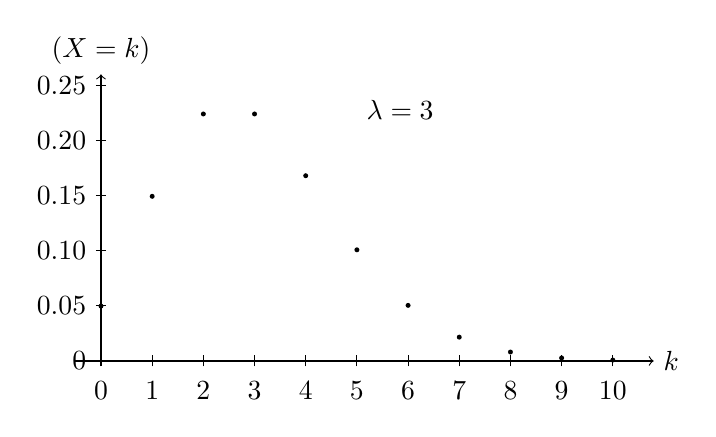
\begin{tikzpicture}[x=0.65cm,y=14cm]
    \draw[->] (-0.5,0) -- (10.8,0) node[right] {$k$};
    \draw[->] (0,0) -- (0,0.26) node[above] {$\bP(X=k)$};
    
    % y轴刻度标注
    \foreach \y in {0, 0.05, 0.10, 0.15, 0.20, 0.25} {
        \draw (-0.1,\y) -- (0.1,\y);
        \node[left] at (-0.1,\y) {\y};
    }
    
    % x轴刻度标注
    \foreach \x in {0, 1, 2, 3, 4, 5, 6, 7, 8, 9, 10} {
        \draw (\x,-0.005) -- (\x,0.005);
        \node[below] at (\x,-0.01) {\x};
    }
    
    % \lambda=3 时, k=0..10 的 pmf 数值(避免 pgfmath 阶乘/幂运算溢出)
    \foreach \kv/\pv in {
        0/0.04979,
        1/0.14936,
        2/0.22404,
        3/0.22404,
        4/0.16803,
        5/0.10082,
        6/0.05041,
        7/0.02160,
        8/0.00810,
        9/0.00270,
        10/0.00081
    } {
        \fill (\kv,\pv) circle (0.9pt);
    }
    \node[above right] at (5,0.21) {$\lambda=3$};
\end{tikzpicture}
\end{center}
\begin{remark}
当 \(n\to\infty\) 时, 
\(\text{Bin}(n, \lambda/n)\) 的 distribution 
趋近于 \(\text{Poi}(\lambda)\).\\
考虑 $X \sim B\left(n, \frac{\lambda}{n}\right)$, 对于固定的 $k$:
$$
\bP(X=k)=\binom{n}{k}\left(\frac{\lambda}{n}\right)^k\left(1-\frac{\lambda}{n}\right)^{n-k}
$$
展开组合数 $\binom{n}{k}$:
$$
\bP(X=k)=\frac{n(n-1) \ldots(n-k+1)}{k!} \cdot \frac{\lambda^k}{n^k} \cdot\left(1-\frac{\lambda}{n}\right)^n \cdot\left(1-\frac{\lambda}{n}\right)^{-k}
$$
重组项:
$$
\bP(X=k)=\frac{\lambda^k}{k!} \cdot \underbrace{\frac{n(n-1) \ldots(n-k+1)}{n^k}}_{(1)} \cdot \underbrace{\left(1-\frac{\lambda}{n}\right)^n}_{(2)} \cdot \underbrace{\left(1-\frac{\lambda}{n}\right)^{-k}}_{(3)}
$$
其中, (1) 的 limit 是 1, 
(2) 的 limit 是 $e^{-\lambda}$, (3) 的 limit 是 1, 因而 
\[
\lim_{n\to\infty} \mathbb{P}(X=k)= e^{-\lambda} \frac{\lambda^k}{k!}
\]
这个极限行为的意义是:
\begin{itemize}
    \item \(\lambda \) 表示: 在一个固定时间/空间窗口内, 一个事件出现的平均次数的观测.
    \item 我们把这段时间间分成 \(n\) 个小窗口, 将这个观测作为先验知识用来 model 这类事件实现的平均概率, 那么
     每个小窗口内事件出现的概率是 \(p = \lambda/n\).  
    \item 每个 \(\text{Bin}(n,\lambda / n)\) 都表示: 在时间细分成
     \(n\) 个小窗口的情况下, 这个事件出现的次数的分布. (注意不是在时间上的分布, 而是在次数上的分布)
    \item 当 \(n\to\infty\) 时, 其意义: 基于连续时间的估计, 
    这个事件在原固定事件窗口内出现的次数的分布. 这就是 
    \(\text{Poi}(\lambda)\) 的意义.
\end{itemize}
因而 Poisson distribution 的意义本质上是: 
\textbf{
给定对一个事件在固定窗口下出现的平均次数的观测(估计), 
那么这个事件在这个窗口内出现 \(n\) 次 
(\(n = 0,1,2,\cdots  \))的概率是多少?}\\
所以 Poisson 分布, 即是\textbf{根据一个事件在给定 windows 内发生次数的 expectation, 来估计这个事件在该 windows 内发生次数的分布的标准方法.}  \\
\end{remark}

\begin{remark}
Further remark: Poisson distribution 的用途.
\begin{itemize}
    \item 它是 model "大量级的小概率事件" 的通用模型.\\ 
    即一段时间内, 一件事情的发生的概率非常小 (\(p \ll 1\)), 
    但是有很多机会发生 (\(n \gg 1\)). 比如放射性衰变.
    \item 现实世界中, 对于一些事情, 我们想要 model 其在一段时间内发生的总次数 (\(n\)) 和单次成功率 (\(p\)) 
    是很困难的. 比如统计今天路过百货大楼的总人数 (\(n\)), 以及每个人路过百货大楼时走进去的概率 (\(p\)). 但是我们
    很容易可以知道: \(\lambda = np\) 的观测. 即: 每天平均有多少人走进百货大楼. 那么我们就可以用 Poisson distribution 来 model 这件事情在一天内发生的次数的分布.\\
\end{itemize}
\end{remark}
\end{example}






\section{continuous random variables}

\subsection{normal random variables}
(5.2 in book)
\begin{definition}
我们称 $X$ is \textbf{normally distributed with parameter $\mu$ and $\sigma$}, if the pdf of $X$ is given by: \[
\rho(x) = \frac{1}{\sigma \sqrt{2\pi}} e^{-\frac{(x - \mu)^2}{2 \sigma ^2}}
\]
写作: \[
X \sim \mathcal{N}(\mu, \sigma^2)
\]
\end{definition}
特别地, 当 $\mu =0, \sigma = 1$ 时, \[
X \sim \mathcal{N}(0, 1)
\]被称为 \textbf{standard normal distribution.}


容易验证: \(\int_{\mathbb{R}} \rho  = 1 \)

\[
I := \int_ 0^\infty e^{\frac{-y^2}{2}} \; dy
\]
\[
I^2 = \Bigg(\int_ 0^\infty e^{\frac{-y^2}{2}} \; dy\Bigg)\Bigg(\int_ 0^\infty e^{\frac{-x^2}{2}} \; dx\Bigg) = \int
\]






rescaling to std normal distribution: 
Suppose \[
Y \sim \mathcal{N}(\mu, \sigma^2)
\] we define \[
X : = \frac{Y - \mu}{\sigma}
\]
Then we have: \[
X \sim \mathcal{N}(0,1)
\]
这是容易验证的. 因为: \[
X \in B \;\; \Longleftrightarrow  \;\; \frac{Y-\mu}{\sigma} \in B \;\; \Longleftrightarrow  \;\; Y \in \sigma B + \mu
\]
因而 \[
P(X \in B ) = P(Y \in \sigma B + \mu)
\]






\subsection{expectation and variance of normal dist}
Suppose $ X \sim \mathcal{N}(0,1)$. Then \[
\mathbb{E}(X) =  \frac{1}{\sqrt{2\pi }} \int _{\mathbb{R}} x   e^{-\frac{x^2}{2}}    \; dx   = 0
\]
since this is \textbf{odd function}.

And  \begin{align}
    \mathbb{E}(X^2) &=  \frac{1}{\sqrt{2\pi }} \int _{\mathbb{R}} x^2   e^{-\frac{x^2}{2}}    \; dx   \\
    &= \frac{1}{\sqrt{2\pi }} \int _{\mathbb{R}} x (x  e^{-\frac{x^2}{2}})    \; dx \\
    &= \frac{1}{\sqrt{2\pi }} \int _{\mathbb{R}} x   ( e^{-\frac{x^2}{2}} )'   \; dx   \\
    & = - \frac{1}{\sqrt{2\pi }}  x e^{-\frac{x^2}{2}} \bigg|^\infty_{-\infty}  +  \frac{1}{\sqrt{2\pi }} \int _{\mathbb{R}}  e^{-\frac{x^2}{2}}    \; dx \\
    &= 0 + 1 = 1
\end{align}

从而: \[
Var(X) = 1
\]




For general normally distributed $Y$, 我们知道了 $X : = \frac{Y - \mu}{\sigma}$ 的 $\mathbb{E}(X)  = 0$, $Var(X) = 1$, 因而 \[
\mathbb{E}(Y) = \mathbb{E}(\sigma X + \mu)   = \mu
\]
\[
Var(Y)  = Var(\sigma X + \mu) =  \mathbb{E}[(\sigma X + \mu - \mu)^2] = \mathbb{E} (\sigma^2 X^2) = \sigma^2 \mathbb{E}[X^2] = \sigma^2 
\]

\begin{remark}
    对于 normally distributed $X$, 
    \[ \mathbb{E}(X^k) =  \frac{1}{\sqrt{2\pi}} \int_\mathbb{R} x^k  e^{-\frac{x^2}{2}}  \; dx  \]
    For $k$ odd, it is $0$.\\
    For $k$ even:
  \begin{align}
      \mathbb{E}(X^k) &=  \frac{1}{\sqrt{2\pi}} \int_\mathbb{R} x^{k-1} (x e^{-\frac{x^2}{2}})  \; dx  \\
      & = -\frac{1}{\sqrt{2\pi}} \int_\mathbb{R} x^{k-1} ( e^{-\frac{x^2}{2}}) ' \; dx \\
      &= 0 + \frac{1}{\sqrt{2\pi}} \int_\mathbb{R} (x^{k-1})' e^{-\frac{x^2}{2}} \;dx \\
      & = \frac{k-1}{\sqrt{2\pi}} \int_\mathbb{R} x^{k-2} e^{-\frac{x^2}{2}} \;dx  \\
      & = (k-1) \mathbb{E}(X^{k-2})
   \end{align}  
   从而: \[
   \mathbb{E(X^k )} = \begin{cases}
       0 ,\quad k = 2j-1 \\
       (2j-1)(2j-3)\cdots 1 = \frac{(2j)!}{2^j j!},\quad k=2j
   \end{cases}
   \]
\end{remark}




\subsection{cdf of normal distribution}
Let $X$ be the std normal distribution.\\
Its cdf given by: \[
\Phi(a) :=F_X(a)  = \int_{(-\infty,a]} \rho(x) \; dx = \frac{1}{\sqrt{2\pi}} \int_{(-\infty,a]}  e^{-\frac{x^2}{2}} \; dx
\]
Important numerical values:
\[
\Phi(-3) \approx 0.0013
\] 
\[
\Phi(-2) \approx 0.023
\]
\[
\Phi(-1) \approx 0.159
\]


Note 由于 $\rho$ (std) 是一个 even function, 有 \(P(X < -1) = P(X>1)\)
因而 \[
P(X \text{ is one std dev from mean}) = 2(P(X < -1)) = 2 \Phi(-1) \approx0.32 = 32\%
\]
Similarly, \[
P(X \text{ is two std dev from mean}) \approx 0.046 = 4.6\%
\]\[
P(X \text{ is three std dev from mean}) \approx 0.0026 = 0.26\%
\]

为什么 normal random variables 非常重要: comes from a "universality property" called \textbf{central limit theorem.} (will be covered later). Now we state a special case: 




Let $S_n$ be 投掷 $n$ 次 $p$-coin 中得到的 $\#$heads. 即 \[
P(H) := p
\]
我们已经知道, $S_n$ 是一个 binomial discrete random variable. 且有 \[
\mathbb{E}(S_n) = np, \quad  Var(S_n) = npq, \quad \sigma(S_n) = \sqrt{npq}
\]

 
\begin{theorem}{DeHavre's Central limit theorem}
    \[
    \lim_{n\to \infty} P\Bigg( \frac{S_n - \mathbb{E}(S_n)}{\sigma(S_n)} \in (a,b)\Bigg) = \Phi(b) - \Phi(a) = \frac{1}{\sqrt{2\pi}} \int_{(a,b)} e^{-\frac{x^2}{2}} \; dx
    \]
\end{theorem}




Write $S_n$ into $n$ 个 i.i.d. random variables
\[
S_n = \sum_{i=1}^n X_i
\]
each $X_i$ 都是一个 trial of tossing the $p$-coin.\\



\begin{example}
    Toss a million times 一个 fair coin. Approximate the prob that we get more than $501000$ heads: 
    \[
    \mathbb{E}(S_{1000000}) = np = 500000
    \]
    \[
    \sigma(S_{1000000}) = \sqrt{npq} = 500
    \] 因而: \[
    P(S_{1000000} > 501000) = P(S_{1000000} - \mathbb{E}(S_{1000000}) > 1000) = P(\frac{S_{1000000} - \mathbb{E}(S_{1000000})}{\sigma(S_{1000000})} > \frac{1000}{500}) = 1-\Phi(2) = \Phi(-2)  \approx 0.159  
    \]
\end{example}



(5.3 in book.)
\subsection{exponential random variables}

我们称 $X$ 为一个 exponential random variable with parameter $\lambda$, 如果它的 pdf is given by: \[
f(x) = \begin{cases}
    \lambda e^{-\lambda x}, \quad x > 0\\
    0, \quad x \leq 0
\end{cases}
\]


Distribution function given by: \[
F_X(x) = \begin{cases}
    \int _{-\infty}^x f(t) \; dt = \lambda \int_0 ^x e^{-\lambda t} \; dt = 1 - e^{-\lambda x}, \quad x> 0\\
    0,\quad x<0
\end{cases}
\]
容易验证, $F_X(x) =0$ when $x \to -\infty$, 以及 $F_X(x) \to 1$ when $x \to \infty$

\begin{align}
P(X> 0)& = 1 - P(X<0)      \\
&= 1- F_X(a) \\
&= e^{-\lambda a}
\end{align}


Expectation and moments: 
We compute the moment $\mathbb{E}[X^n], \quad n\geq 0$

$\mathbb{E}[X^0] = \mathbb{E}[1] = 1$

\begin{align}
\mathbb{E}[X^n] &= \lambda \int_0^\infty x^n e^{-\lambda x } \; dx  \\
&= - \int_0 ^\infty  x^n(e^{-\lambda x})' \; dx \\
&=  0 + \int_0 ^\infty n x^{n-1} e^{-\lambda x} \; dx \\
&= \frac{n}{\lambda} \mathbb{E}(X^{n-1})
\end{align}

因而 recursively get: \[
\mathbb{E}[X^n] = \frac{n!}{\lambda^n}
\]

\(\mathbb{E}[X] = \frac{1}{\lambda}, \mathbb{E}[X^2] = \frac{2}{\lambda^2}, \cdots  \)


从而: \[
Var[X] = \frac{2}{\lambda^2} - \frac{1}{\lambda^2} = \frac{1}{\lambda^2}
\]


Recall the Gamma function: \[
n!  = \int_0^\infty x^n e^{-x} \; dx  = \Gamma(n+1) \]


Interpretation: \textbf{exponential r.v. 是 geometric r.v. 的 continuous analogue.}


First time to get heads in a seq of Bernoulli coins:
\begin{align}
    p(k) &= (1-p)^{k-1} p  \\
    &= (1-p)^k \frac{p}{1-p}
\end{align}
如果我们令 $e^{-\lambda} := 1-p$
就得到: \[
p(k) = e^{-\lambda k} \frac{p}{1-p} 
\]
和 discrete 的 geometric distribution 相似, exponential distribution 是用来 \textbf{model the first time an event occurs}.


\begin{example}
    Suppose 一个 storage battery 的 lifetime 是 exponentially distributed 的, 并且 average 为 10 hours. Suppose 我们想要 use this battery for 5 hours for.
计算: probability of finishing the task, if:\\ 
(a) 使用一个 new battery\\
(b) 使用一个已经用过 2 hours 的 battery\\
\begin{solution}
    \[
    \mathbb{E}[X] = 10 = \frac{1}{\lambda} \implies \lambda = \frac{1}{10}
    \]
如果我们使用一个 new battery, 则 want: $P(X>5) = 1 - P(X<5) = 1- F_X(5) = e^{-\frac{1}{2}}$
如果我们使用一个用过 2 hours 的 battery, 则 want: \[
P(X> 5+2 \mid X > 2) = \frac{e^{-(5+2)\lambda}}{e^{-2\lambda }} = e^{-5\lambda} = = e^{-\frac{1}{2}}
\]
\end{solution}

Notice: 我们发现 \[
P(X>5) = P(X> 5+2 \mid X > 2)
\]
\end{example}

\begin{theorem}
一 ctn r.v. 有: \[
    P(X > b+ t \mid X > b) = P(X>t)
    \]
\textbf{当且仅当它是一个 exponential random variable.}
\end{theorem}
\begin{remark}
    "如果 $X$ 表示某个 event 发生的时间, 在已经过去时间 $b$ 而没发生的情况下, 再过时间 $t$ 发生这个时间的条件概率, 等于从时间 $0$ 开始, 过时间 $t$ 发生这个事件的初始概率."\\
    并且 notice 这是一个 iff statement
\end{remark}

\begin{proof}
\begin{align}
     &   P(X > b+ t \mid X > b) = P(X>t) \\
   \Longleftrightarrow  & P(X > b+t) = P(X > t) P(X>b) \\
    \Longleftrightarrow  & X \text{ exponential (check) }
\end{align}
\end{proof}





\subsection{Gamma distribution}

\begin{definition}{$\Gamma$-distribution}
Recall $\Gamma$ function: \[
    \Gamma(\alpha) = \int_0^\infty x^{\alpha - 1} e^{-x}\; dx
    \]
一个 ctn r.v. 被称为 have Gamma distribution with parameter $\alpha, \lambda$, 写作 $X \sim \Gamma(\alpha, \lambda)$, (其中 $\alpha > 0, \lambda > 0$), 如果它的 pdf 为 \[
f(x) = \begin{cases}
    \frac{\lambda e^{-\lambda x} (\lambda x)^{\alpha -1} }{\Gamma (\alpha)}, \quad x>0 \\
    0, \quad x \leq 0
\end{cases}
\]
\end{definition}
\begin{remark}
我们已经知道, $\Gamma$ 函数是对 define 在自然数上的 factorial 函数, 推广到 defined 在 $[0,\infty)$ 上.
我们有:  \[
\Gamma(\alpha + 1) = \alpha \Gamma(\alpha)
\]\[
n! = \Gamma(n+1)
\]
\end{remark}


Interpretation: $\Gamma$ distribution 的 random variable 是 binomial random variable 的 ctn version.

考虑 $\alpha : = n$ 为一个正整数, 那么它可以用来 model the first time an event occurs in a Poission process.

Expectation:  \begin{align}
    \mathbb{E}[X] &= \frac{1}{\Gamma(\alpha)} \int_0^\infty (\lambda x )^{\alpha -1} \lambda  e^{-\lambda x} \; dx\\
    &=  \frac{1}{\lambda \Gamma(\alpha)}  \int_0^\infty x^\alpha e^{-x} \; dx \\
    &= \frac{\Gamma(\alpha + 1)}{\lambda \Gamma(\alpha)} = \frac{\alpha}{\lambda}
\end{align}
(since $\Gamma(\alpha + 1) = \alpha \Gamma(\alpha)$.)

我们可以计算得: \[
\mathbb{E}[X^2] = \frac{\alpha}{\lambda^2}
\]

\subsection{Cauchy distribution}
\begin{definition}
    一个 random variable 被称为 have Cauchy distribution with parameter $\theta \in \mathbb{R}$, 如果它的 pdf 是: \[
    f(x)   =\frac{1}{\pi} \frac{1}{1+(x-\theta)^2} , \quad x\in \mathbb{R}
    \]
    当 $\theta = 0$ 时, 被称为 standard Cauchy distribution.
\end{definition}


CDF: \begin{align}
    F_X(a) = \int_{-\infty}^a f(x) \; dx &= \frac{1}{\pi} \int_0^\infty \frac{1}{1+ (x-\theta)^2} \; dx \\ 
    &= \frac{1}{\pi} \int_0^\infty  \frac{1}{1+ y^2} \; dy \\
    &= \frac{1}{\pi} \arctan y \Big|_{\infty}^{a - \theta} \\
    &=  \frac{1}{\pi} (\arctan (a - \theta) + \frac{\pi}{2}) \\
    &= \frac{1}{\pi} \arctan (a - \theta) + \frac{1}{2}
\end{align}

\begin{example}
A macro-beam flashlight is spin around tis center located at $(0,1)$.\\
假设 the angle of the flashlight is uniform in $(-\frac{\pi}{2}, \frac{\pi}{2})$, 并令 $X$ 为 the point on $x$-axis where the beam hits.\\
The distribution function of $X$ is: \[
F_X(a) = P(X < a) = P(\tan \alpha < a) = P(\alpha < \arctan a)
\]
因而 $X$ 为一个 std Cauchy r.v.  
\end{example}

Interpretation: Brownian motion models (among many other things) the motion of small particles, 比如气体和液体分子.\\

FACT: 如果 start the Brownian motion at $(0,1)$, 并令 $X $ 表示 the first point that the motion hits the $x$-axis, 那么 $X$ 为一个 std Cauchy r.v.  




\begin{remark}
Distribution of a function of a random variable: \\
令 $F_X$ 为一个 r.v. $X$ 的 cdf.\\
考虑 $Y := X^3$.\\
那么 $Y$ 的 distribution 是什么? \[
F_Y(a) = P(X^3 < a ) = P(X < a^3) = F_X(a^{1/3})
\]
更加 generally, 如果 \[
Y: = g(X)
\]
where $g$ 是一个 $\mathbb{R}\to \mathbb{R}$ 的 measurable function. \\
那么: \[
F_Y(a) = P(g(x) < a) = F_X(g^{-1} (a) )
\]
并且 pdf of $Y$: 
\begin{align}
\rho_y(x)  = \frac{d}{ dx} F_y(x) &= \frac{d}{dx} F_X(g^{-1}(a)) \\
&= F_X(g^{-1}(x)) \frac{d}{dx} g^{-1}(x) \\
&= f_x(g^{-1}(x)) \frac{d}{dx} g^{-1}(x)
\end{align}

\end{remark}












\section{independence}



% \chapter*{Homework 2}
\section*{Problem 1}
Suppose that the cumulative distribution function (CDF) of a random variable $F: \mathbb{R} \rightarrow \mathbb{R}$ is strictly increasing and continuous. Let $U$ be a random variable with the uniform distribution on $(0,1)$ and define
$$
X:=F^{-1}(U) .
$$
Show that $X$ has CDF equal to $F$.
This exercise shows us how to construct a random variable with given distribution, assuming that we have a uniform random variable.
\begin{proof}
Since $F$ is strictly increasing and continuous, it has an inverse function $F^{-1}$ on its range, and $F^{-1}$ is also strictly increasing.

For any $x \in \mathbb{R}$, we have
\[
\{X \le x\}=\{F^{-1}(U)\le x\}.
\]
Since $F^{-1}$ is strictly increasing, the above is equivalent to
\[
\{U \le F(x)\}.
\]
Therefore
\[
\mathbb{P}(X \le x)=\mathbb{P}(U \le F(x)).
\]
Since $U \sim \mathrm{Unif}(0,1)$ and for a CDF we have $F(x)\in[0,1]$, we get
\[
\mathbb{P}(U \le F(x)) = F(x).
\]
Thus for all $x$, the CDF of $X$ satisfies $\mathbb{P}(X \le x)=F(x)$, i.e., the CDF of $X$ equals $F$.
\end{proof}


\section*{Problem 2}
A gas station fills its tank completely once a week. 
Let the weekly sales volume (in thousands of liters) be a random variable with density
$$
f(x)= \begin{cases}a(1-x)^4, & x \in(0,1), \\ 0, & \text { otherwise } .\end{cases}
$$
Find the constant $a$. What should be the tank capacity 
so that the probability of running out of fuel during a given week is $1 / 100$ ?
\begin{solution}
(1) Since the density integrates to 1,
\[
1=\int_{-\infty}^{\infty} f(x)\,dx=\int_0^1 a(1-x)^4\,dx
= a \int_0^1 (1-x)^4\,dx.
\]
Let $u=1-x$, then $\int_0^1 (1-x)^4 dx=\int_0^1 u^4 du=\frac{1}{5}$, so $a\cdot \frac{1}{5}=1$, which gives
\[
a=5.
\]

(2) Let the tank capacity be $c$ (in thousands of liters). Running out of fuel in a week occurs when sales exceed $c$, i.e., the event $\{X>c\}$. We need
\[
\mathbb{P}(X>c)=\frac{1}{100}.
\]
Since $a=5$,
\[
\mathbb{P}(X>c)=\int_c^1 5(1-x)^4\,dx.
\]
Again let $u=1-x$, then when $x=c$ we have $u=1-c$, when $x=1$ we have $u=0$, so
\[
\int_c^1 5(1-x)^4 dx = 5\int_{1-c}^{0} u^4(-du)=5\int_0^{1-c} u^4 du
=5\cdot \frac{(1-c)^5}{5}=(1-c)^5.
\]
Therefore
\[
(1-c)^5=\frac{1}{100} \quad \Longrightarrow \quad 1-c=\left(\frac{1}{100}\right)^{1/5}=100^{-1/5}=10^{-2/5},
\]
thus
\[
c=1-10^{-2/5}.
\]
So the tank capacity should be $\bigl(1-10^{-2/5}\bigr)$ thousand liters, i.e., $1000\bigl(1-10^{-2/5}\bigr)$ liters.
\end{solution}





\section*{Problem 3}
Let the random variable $X$ have density
$$
f_X(x)= \begin{cases}\frac{1}{2 x^2}, & |x| \geq 1, \\ 0, & |x|<1 .\end{cases}
$$
Find the probability density function of $Y:=X^2$ and 
compute the probability $\mathbb{P}(2 Y+3 \leq 10)$.
\begin{solution}
Since $Y=X^2$, we have $Y\ge 1$. For $y\ge 1$, the transformation $y=x^2$ has two preimages $x=\sqrt{y}$ and $x=-\sqrt{y}$, and
\[
\left|\frac{dx}{dy}\right|=\frac{1}{2\sqrt{y}}.
\]
Therefore
\[
f_Y(y)= f_X(\sqrt{y})\frac{1}{2\sqrt{y}} + f_X(-\sqrt{y})\frac{1}{2\sqrt{y}}, \quad y\ge 1.
\]
Since $f_X(\pm \sqrt{y})=\frac{1}{2(\sqrt{y})^2}=\frac{1}{2y}$, we get
\[
f_Y(y)=\frac{1}{2y}\cdot\frac{1}{2\sqrt{y}}+\frac{1}{2y}\cdot\frac{1}{2\sqrt{y}}
= \frac{1}{2y^{3/2}}, \quad y\ge 1,
\]
and $f_Y(y)=0$ when $y<1$. That is,
\[
f_Y(y)=
\begin{cases}
\dfrac{1}{2y^{3/2}}, & y\ge 1,\\[6pt]
0, & y<1.
\end{cases}
\]

Next,
\[
\mathbb{P}(2Y+3\le 10)=\mathbb{P}\!\left(Y\le \frac{7}{2}\right)
= \int_{1}^{7/2} \frac{1}{2y^{3/2}}\,dy.
\]
Evaluating the integral:
\[
\int \frac{1}{2}y^{-3/2}dy=\frac{1}{2}\cdot\left(-2y^{-1/2}\right)=-y^{-1/2},
\]
therefore
\[
\mathbb{P}\!\left(Y\le \frac{7}{2}\right)
=\left[-y^{-1/2}\right]_{1}^{7/2}
=1-\frac{1}{\sqrt{7/2}}
=1-\sqrt{\frac{2}{7}}.
\]
\end{solution}






\section*{Problem 4}
Let the random variable $X$ have density $f$, 
which is symmetric about $\mu \in \mathbb{R}$, 
that is, $f(\mu+x)= f(\mu-x)$, for all $x \in \mathbb{R}$. 
Show that $\mathbb{P}(X \leq \mu)=\mathbb{P}(X \geq \mu)$. 
If in addition $\mathbb{E}|X|<\infty$, show that $\mathbb{E}(X)=\mu$.
 Can you use this observation if $X \sim N(0,1)$ ?
\begin{proof}
(1) Since $X$ has density $f$, we have $\mathbb{P}(X=\mu)=0$, and
\[
\mathbb{P}(X\le \mu)=\int_{-\infty}^{\mu} f(x)\,dx,\qquad
\mathbb{P}(X\ge \mu)=\int_{\mu}^{\infty} f(x)\,dx.
\]
For the first integral, substitute $x=\mu-t$, then $dx=-dt$. When $x\to -\infty$ we have $t\to \infty$, when $x=\mu$ we have $t=0$, so
\[
\int_{-\infty}^{\mu} f(x)\,dx
=\int_{\infty}^{0} f(\mu-t)(-dt)
=\int_{0}^{\infty} f(\mu-t)\,dt.
\]
By symmetry $f(\mu-t)=f(\mu+t)$, so
\[
\int_{0}^{\infty} f(\mu-t)\,dt=\int_{0}^{\infty} f(\mu+t)\,dt
=\int_{\mu}^{\infty} f(x)\,dx.
\]
Therefore $\mathbb{P}(X\le \mu)=\mathbb{P}(X\ge \mu)$.

(2) If $\mathbb{E}|X|<\infty$, then $\mathbb{E}|X-\mu|<\infty$, and
\[
\mathbb{E}(X-\mu)=\int_{-\infty}^{\infty} (x-\mu)f(x)\,dx.
\]
Let $t=x-\mu$, then
\[
\mathbb{E}(X-\mu)=\int_{-\infty}^{\infty} t\, f(\mu+t)\,dt.
\]
By symmetry $f(\mu+t)=f(\mu-t)$, the function $g(t):=t f(\mu+t)$ is odd, since
\[
g(-t)=(-t)f(\mu-t)=(-t)f(\mu+t)=-g(t).
\]
Under the condition that the expectation exists (absolutely integrable), the integral of an odd function over a symmetric interval is 0, so
\[
\mathbb{E}(X-\mu)=0 \quad \Longrightarrow \quad \mathbb{E}(X)=\mu.
\]

(3) If $X\sim N(0,1)$, its density is symmetric about $\mu=0$ and $\mathbb{E}|X|<\infty$, so we can apply the above result to get $\mathbb{E}(X)=0$.
\end{proof}





\section*{Problem 5}
An airline has observed that $5 \%$ of ticket holders do not show up for their flight. Today's flight has an airplane with 200 seats, and the airline has sold 203 tickets.
What is the probability that the airline will not be able to accommodate a ticketed passenger? Assume that, for each passenger $i$, 
the event $A_i$ that passenger $i$ shows up is independent of all others,
for $1 \leq i \leq 203$.
\begin{solution}
Let the random variable $S$ denote the number of passengers who actually show up among the 203 ticket holders. Then $S\sim \mathrm{Bin}(n=203,p=0.95)$.

The airline cannot accommodate ticketed passengers if and only if the number of passengers who show up exceeds the 200 seats, i.e., the event $\{S\ge 201\}$. Therefore the required probability is
\[
\mathbb{P}(S\ge 201)=\sum_{k=201}^{203} \binom{203}{k}(0.95)^k(0.05)^{203-k}.
\]
Numerically,
\[
\mathbb{P}(S\ge 201)\approx 0.002058,
\]
which is approximately $0.2058\%$.
\end{solution}


\section*{Problem 6}
Consider a sequence of tosses of a fair die. We continue tossing until both outcomes 3 and 4 have appeared at least once. For example, 
one possible sequence of results is
$$
5,1,1,4,6,5,4,2,6,3,
$$
and we then stop. Let $X$ be the number of tosses required (in this example, $X=10$ ).
What is the expected value of the random variable $X$ ?
\begin{solution}
We use states to characterize the appearance of $\{3,4\}$:

Let $E_0$ be the expected number of tosses needed from the initial state (neither 3 nor 4 has appeared) to the end.
Let $E_1$ be the expected number of tosses needed from the state where one of them has appeared (only 3 or only 4 has appeared) to the end.

First, find $E_1$. In state 1, each toss has probability $1/6$ of getting the missing number and thus ending, and probability $5/6$ of remaining in state 1. Therefore
\[
E_1 = 1 + \frac{5}{6}E_1 + \frac{1}{6}\cdot 0
\quad \Longrightarrow \quad
E_1 = 6.
\]

Next, find $E_0$. In state 0, each toss:
has probability $2/6$ of getting 3 or 4 and thus entering state 1,
has probability $4/6$ of getting other numbers and thus remaining in state 0. So
\[
E_0 = 1 + \frac{4}{6}E_0 + \frac{2}{6}E_1.
\]
Substituting $E_1=6$:
\[
E_0 = 1 + \frac{4}{6}E_0 + \frac{2}{6}\cdot 6
= 1 + \frac{4}{6}E_0 + 2.
\]
Rearranging gives
\[
\left(1-\frac{4}{6}\right)E_0 = 3
\quad \Longrightarrow \quad
\frac{2}{6}E_0 = 3
\quad \Longrightarrow \quad
E_0 = 9.
\]
Therefore $\mathbb{E}[X]=9$.
\end{solution}
 \chapter*{Homework 3}
\section*{Problem 1}
Let $Z$ be a standard normal random variable $Z \sim N(0,1)$. We denote by $\Phi$ its distribution function. Answer the questions below
\begin{itemize}
    \item [(a)] If $a, b \in \mathbb{R}$ with $a>0$, show that the random variable $a Z+b$ 
    is also normal and find its mean and variance.
    \item [(b)] Show that $\Phi(0)=1 / 2$.
    \item [(c)] Show that $\Phi(-x)=1-\Phi(x)$ for any $x \in \mathbb{R}$.
\end{itemize}
\begin{solution}
\begin{itemize}
\item [(a)]
$Z\sim N(0,1)$ has density
\[
f_Z(z)=\frac{1}{\sqrt{2\pi}}e^{-z^2/2}
\]

\begin{align*}
    F_X(x) =\bP(X \leq x) &= \bP(aZ+b \leq x) \\
    &= \bP\left(Z \leq \frac{x-b}{a}\right) \\
    & = \Phi\left(\frac{x-b}{a}\right)
\end{align*}
Thus \[
f_X(x) = \frac{d}{dx} \Phi\left(\frac{x-b}{a}\right) =
 \frac{1}{a} \varphi\left(\frac{x-b}{a}\right) = 
 \frac{1}{\sqrt{a^22\pi}} e^{-\frac{(x-b)^2}{2a^2}}
\]

Note this is the density of a normal distribution with mean $b$ and variance $a^2$. 
Therefore
\[
aZ+b \sim N(b,a^2)
\]
Since $Z$ has mean $0$ and variance $1$, use linearity we have
\[
\mathbb E[aZ+b]=a\mathbb E[Z]+b=b
\]
and 
\[
\mathrm{Var}(aZ+b)=a^2\mathrm{Var}(Z)=a^2
\]
\item [(b)] 
Note the standard normal density is an even function:
\[
\varphi(x)=\frac{1}{\sqrt{2\pi}}e^{-x^2/2} = \varphi(-x)
\]
Thus
\[
\Phi(0)=\int_{-\infty}^{0}\varphi(x)\,dx
=\int_{0}^{\infty}\varphi(x)\,dx
\]
Since $\int_{-\infty}^{\infty}\varphi(x)\,dx=1$, 
the two equal halves are each $1/2$, so $\Phi(0)=1/2$.
\item [(c)]
For any $x\in\mathbb R$,
\[
\Phi(-x)=\int_{-\infty}^{-x}\varphi(t)\,dt
\]
Let $u=-t$, using $\varphi(-u)=\varphi(u)$ we have
\[
\Phi(-x)=\int_{\infty}^{x}\varphi(-u)(-du)=\int_{x}^{\infty}\varphi(u)\,du
=1-\int_{-\infty}^{x}\varphi(u)\,du
=1-\Phi(x)
\]
\end{itemize}

\end{solution}





\section*{Problem 2}
Let $X$ and $Y$ be random variables with joint density
$$
f(x, y)= \begin{cases}-x y, & (x, y) \in(-1,0) \times(0,1) \cup(1,2) \times(-1,0), \\ 0, 
& \text { otherwise }\end{cases}
$$
\begin{itemize}
    \item [(a)] Compute the probability $\mathbb{P}(X+Y<0)$.
    \item [(b)] Compute the expected value $\mathbb{E}[X Y]$.
    \item [(c)] Are $X$ and $Y$ independent?
\end{itemize}
\begin{solution}
\begin{itemize}
\item [(a)]
On $(1,2)\times(-1,0)$ we have $x+y>0$ since $x>1$ and $y>-1$, 
hence this region contributes nothing to $\{X+Y<0\}$.

On $(-1,0)\times(0,1)$, the ineq $x+y<0$ is equivalent to $0<y<-x$. Therefore,
\[
\mathbb P(X+Y<0)=\int_{-1}^{0}\int_{0}^{-x} (-xy)\,dy\,dx
\]
Compute the inner integral:
\[
\int_{0}^{-x} (-xy)\,dy=-x\cdot \frac{(-x)^2}{2}=-\frac{x^3}{2}
\]
Hence,
\[
\mathbb P(X+Y<0)=\int_{-1}^{0}\left(-\frac{x^3}{2}\right)dx
=-\frac12\cdot \frac{x^4}{4}\Big|_{-1}^{0}=\frac18
\]

\item [(b)]
By def,
\begin{align*}
\mathbb E[XY]&=\int_{\bR^2} xy\,f(x,y)\,dx\,dy \\
&=-\int_{(-1,0)\times(0,1)\cup(1,2)\times(-1,0)} x^2y^2\,dx\,dy     \\
&= -\int_{-1}^{0}\int_{0}^{1} x^2y^2\,dy\,dx  - \int_{1}^{2}\int_{-1}^{0} x^2y^2\,dy\,dx
\end{align*}

Split over the two rectangles.
On $(-1,0)\times(0,1)$,
\[
-\int_{-1}^{0}\int_{0}^{1} x^2y^2\,dy\,dx
=-\left(\int_{-1}^{0}x^2\,dx\right)\left(\int_{0}^{1}y^2\,dy\right)
=-\left(\frac13\right)\left(\frac13\right)=-\frac19
\]
On $(1,2)\times(-1,0)$,
\[
-\int_{1}^{2}\int_{-1}^{0} x^2y^2\,dy\,dx
=-\left(\int_{1}^{2}x^2\,dx\right)\left(\int_{-1}^{0}y^2\,dy\right)
=-\left(\frac73\right)\left(\frac13\right)=-\frac79
\]
Thus,
\[
\mathbb E[XY]=-\frac19-\frac79=-\frac89
\]

\item [(c)]
Consider: For $x\in(-1,0)$,
\[
f_X(x)=\int_{0}^{1}(-xy)\,dy=\frac{-x}{2}
\]
For $y\in(0,1)$,
\[
f_Y(y)=\int_{-1}^{0}(-xy)\,dx=y\int_{-1}^{0}(-x)\,dx=\frac{y}{2}
\]
And for $(x,y)\in(-1,0)\times(0,1)$,
\[
f_X(x)f_Y(y)=\left(\frac{-x}{2}\right)\left(\frac{y}{2}\right)=\frac{-xy}{4}\neq -xy=f(x,y)
\]
Thus $X$ and $Y$ are not independent.
\end{itemize}

\end{solution}


\section*{Problem 3}
Let $X \sim \operatorname{Exp}(1)$ and $Y=X+\frac{1}{X+1}$. 
Find $\mathbb{P}((X+1) Y \leq 2)$ and $\operatorname{Cov}(X, Y)$.\\
Hint: You may leave your answer as a function of the integral $\int_0^{\infty} \frac{e^{-x}}{1+x} d x$.
\begin{solution}
Note 
\[
(X+1)Y=(X+1)\left(X+\frac{1}{X+1}\right)=X(X+1)+1=X^2+X+1
\]
Thus,
\[
(X+1)Y\le 2 \iff X^2+X-1\le 0
\]
The roots of $x^2+x-1=0$ are $\frac{-1\pm \sqrt5}{2}$. Since $X\ge 0$, the event is
\[
0\le X\le \frac{\sqrt5-1}{2}
\]
Therefore, using the CDF of $\mathrm{Exp}(1)$,
\[
\mathbb P((X+1)Y\le 2)=\mathbb P(X\le \frac{\sqrt5-1}{2})=1-e^{-\frac{\sqrt5-1}{2}}
=1-\exp\!\left(-\frac{\sqrt5-1}{2}\right)
\]
Nowe we compute the covariance. By def,
\[
\mathrm{Cov}(X,Y)=\mathbb E[XY]-\mathbb E[X]\mathbb E[Y]
\]
For $X\sim\mathrm{Exp}(1)$, $\mathbb E[X]=1$ and $\mathbb E[X^2]=2$. Let
\[
I:=\int_{0}^{\infty}\frac{e^{-x}}{1+x}\,dx=\mathbb E\!\left[\frac{1}{1+X}\right]
\]
Then
\[
\mathbb E[Y]=\mathbb E[X]+\mathbb E\!\left[\frac{1}{1+X}\right]=1+I
\]
Also,
\[
XY=X\left(X+\frac{1}{1+X}\right)=X^2+\frac{X}{1+X}
=X^2+\left(1-\frac{1}{1+X}\right)
\]
so
\[
\mathbb E[XY]=\mathbb E[X^2]+1-\mathbb E\!\left[\frac{1}{1+X}\right]=2+1-I=3-I
\]
Hence,
\[
\mathrm{Cov}(X,Y)=(3-I)-(1)(1+I)=2-2I
=2-2\int_{0}^{\infty}\frac{e^{-x}}{1+x}\,dx
\]
\end{solution}


\section*{Problem 4}
Find the conditional density $f_{Y \mid X}(y \mid x)$ of $Y$
 given that $X=x$ and the corresponding conditional expectation 
 $\mathbb{E}[Y \mid X=x]$ if the pair of random variables $(X, Y)$ 
 has absolutely continuous distribution with joint density: 
 $f_{X, Y}(x, y)=\lambda^2 e^{-\lambda y} \mathbf{1}_{\{0 \leq x \leq y\}}$.
\begin{solution}
Given the joint density
\(
f_{X,Y}(x,y)=\lambda^2 e^{-\lambda y}\mathbf 1_{\{0\le x\le y\}}
\), we first compute the marginal density of $X$. For $x\ge 0$,
\[
f_X(x)=\int_{y=x}^{\infty}\lambda^2 e^{-\lambda y}\,dy
=\lambda^2\cdot \frac{e^{-\lambda x}}{\lambda}
=\lambda e^{-\lambda x}
\]
and $f_X(x)=0$ for $x<0$.

Therefore, for $x\ge 0$,
\[
f_{Y|X}(y|x)=\frac{f_{X,Y}(x,y)}{f_X(x)}
=\frac{\lambda^2 e^{-\lambda y}\mathbf 1_{\{y\ge x\}}}{\lambda e^{-\lambda x}}
=\lambda e^{-\lambda (y-x)}\mathbf 1_{\{y\ge x\}}
\]
This shows that $Y|X=x$ has the same distribution as $x+E$ where $E\sim \mathrm{Exp}(\lambda)$, hence
\[
\mathbb E[Y|X=x]=x+\frac{1}{\lambda}
\]
\end{solution}



\section*{Problem 5}
A machine produces a coin that shows heads with a random probability $p$. 
The value of $p$ is unknown to us, but from many observations of the coins produced by the machine 
we know that the distribution of the random parameter $p$ is uniform on $(0,1 / 2)$. 
We start tossing the coin. Compute the following probabilities:
\begin{itemize}
    \item [(a)] The coin shows heads on the first toss.
    \item [(b)] The expected number of tosses until tails show up.
\end{itemize}
\begin{solution}

\begin{itemize}
\item [(a)] 
The head probability $p\sim \mathrm{Unif}(0,1/2)$. Thus the density is:
\[
f_P(p)=2\,\mathbf 1_{(0,1/2)}(p)
\]
The unconditional probability of heads on the first toss is
\[
\mathbb P(\text{H on first toss})=\mathbb E[p]
=\int_0^{1/2} p\cdot 2\,dp
=2\cdot \frac{p^2}{2}\Big|_{0}^{1/2}
=\frac14
\]

\item [(b)]
Let $T$ be the number of tosses until the first tail occurs. 
Conditional on $p$, tails occurs with probability $1-p$ each toss, 
so $T$ is geometric with parameter $1-p$.
Hence
\[
\mathbb E[T\,|\,p]=\frac{1}{1-p}
\]
Taking expectation over $p$,
\[
\mathbb E[T]=\mathbb E\!\left[\frac{1}{1-p}\right]
=\int_0^{1/2}\frac{1}{1-p}\cdot 2\,dp
=2\big[-\ln(1-p)\big]_{0}^{1/2}
=2\ln 2
\]
\end{itemize}


\end{solution}


\section*{Problem 6}
The joint probability density function of the random variables $X$ and $Y$ is given by
$$
f_{X, Y}(x, y)= \begin{cases}c\left(x^2+\frac{x y}{2}\right), & (x, y) \in(0,1) \times(0,2) \\ 
0, & \text { otherwise }\end{cases}
$$
\begin{itemize}
    \item [(a)] Find the constant $c$.
    \item [(b)] Find the marginal density of $X$ and compute $\mathbb{E}[X]$.
    \item [(c)] Compute $\mathbb{P}(X>Y)$.
    \item [(d)] Compute $\mathbb{P}\left(\left.Y>\frac{1}{2} \right\rvert\, X<\frac{1}{2}\right)$.  
\end{itemize}
\begin{solution}
\begin{itemize}
\item [(a)]
Determine $c$ from normalization:
\[
1=\int_0^1\int_0^2 c\left(x^2+\frac{xy}{2}\right)\,dy\,dx
\]
For fixed $x$,
\[
\int_0^2\left(x^2+\frac{xy}{2}\right)dy
=2x^2+\frac{x}{2}\cdot\frac{y^2}{2}\Big|_{0}^{2}
=2x^2+x
\]
Thus
\[
1=c\int_0^1(2x^2+x)\,dx
=c\left(\frac{2}{3}+\frac12\right)
=c\cdot\frac{7}{6}
\]
so $c=\frac{6}{7}$

\item [(b)]
The marginal density of $X$ (for $0<x<1$) is
\[
f_X(x)=\int_0^2 c\left(x^2+\frac{xy}{2}\right)\,dy=c(2x^2+x)=\frac{6}{7}(2x^2+x)
\]
and $f_X(x)=0$ otherwise.

Thus
\[
\mathbb E[X]=\int_0^1 x f_X(x)\,dx
=\frac{6}{7}\int_0^1(2x^3+x^2)\,dx
=\frac{6}{7}\left(\frac12+\frac13\right)=\frac{5}{7}
\]

\item [(c)]
The event $\{X>Y\}$ corresponds to the region $0<y<x<1$ (since $x\in(0,1)$). Hence
\[
\mathbb P(X>Y)=\int_0^1\int_0^x c\left(x^2+\frac{xy}{2}\right)\,dy\,dx
\]
For fixed $x$,
\[
\int_0^x\left(x^2+\frac{xy}{2}\right)dy
=x^3+\frac{x}{2}\cdot\frac{y^2}{2}\Big|_{0}^{x}
=x^3+\frac{x^3}{4}=\frac{5}{4}x^3
\]
Therefore
\[
\mathbb P(X>Y)=c\int_0^1\frac{5}{4}x^3\,dx
=c\cdot\frac{5}{4}\cdot\frac14
=c\cdot\frac{5}{16}
=\frac{6}{7}\cdot\frac{5}{16}
=\frac{15}{56}
\]

\item [(d)]
By definition,
\[
\mathbb P\!\left(\left.Y>\frac12\right|X<\frac12\right)
=\frac{\mathbb P\left(Y>\frac12,\ X<\frac12\right)}{\mathbb P\left(X<\frac12\right)}
\]
Calculate each part. First the denominator:
\[
\mathbb P\left(X<\frac12\right)=\int_0^{1/2} f_X(x)\,dx
=c\int_0^{1/2}(2x^2+x)\,dx
=c\left(\frac{1}{12}+\frac18\right)
=c\cdot\frac{5}{24}
=\frac{5}{28}
\]
And the numerator:
\[
\mathbb P\left(Y>\frac12,\ X<\frac12\right)
=\int_0^{1/2}\int_{1/2}^{2} c\left(x^2+\frac{xy}{2}\right)\,dy\,dx
\]
For fixed $x$,
\[
\int_{1/2}^{2}\left(x^2+\frac{xy}{2}\right)dy
=x^2\left(2-\frac12\right)+\frac{x}{2}\cdot\frac{y^2}{2}\Big|_{1/2}^{2}
=\frac{3}{2}x^2+\frac{x}{4}\left(4-\frac14\right)
=\frac{3}{2}x^2+\frac{15}{16}x
\]
Thus
\[
\mathbb P\left(Y>\frac12,\ X<\frac12\right)
=c\int_0^{1/2}\left(\frac{3}{2}x^2+\frac{15}{16}x\right)dx
=c\left(\frac{1}{16}+\frac{15}{128}\right)
=c\cdot\frac{23}{128}
=\frac{69}{448}
\]
Therefore,
\[
\mathbb P\!\left(\left.Y>\frac12\right|X<\frac12\right)
=\frac{69/448}{5/28}
=\frac{69}{80}
\]
\end{itemize}
\end{solution}
\end{document}

